% ----------------------------------------------------------
\chapter{Resultados}
% ----------------------------------------------------------

Esta seção apresenta os resultados obtidos ao longo do desenvolvimento do protótipo de modelador de diagramas ER colaborativo. Os resultados são organizados nas seguintes etapas: o diagrama de caso de uso, os modelos de dados, a arquitetura implementada e as funcionalidades do protótipo.

\section{Diagrama de Caso de Uso}

O diagrama de caso de uso detalha as interações entre os atores e o sistema. Foram identificados três atores distintos, cada um representando um perfil de acesso diferente dentro da plataforma: \textit{Viewer}, \textit{Editor} e \textit{Owner}. A especificação completa de cada caso de uso encontra-se no \hyperref[anx:caso-de-uso]{Anexo A}.

O ator \textit{Viewer}, apresentado na Figura~\ref{fig:caso-de-uso-viewer}, representa o colaborador com acesso somente leitura. Após realizar o \textit{login}, ele pode listar os projetos dos quais faz parte e visualizar os diagramas associados a eles.

\begin{figure}[H]
    \centering
    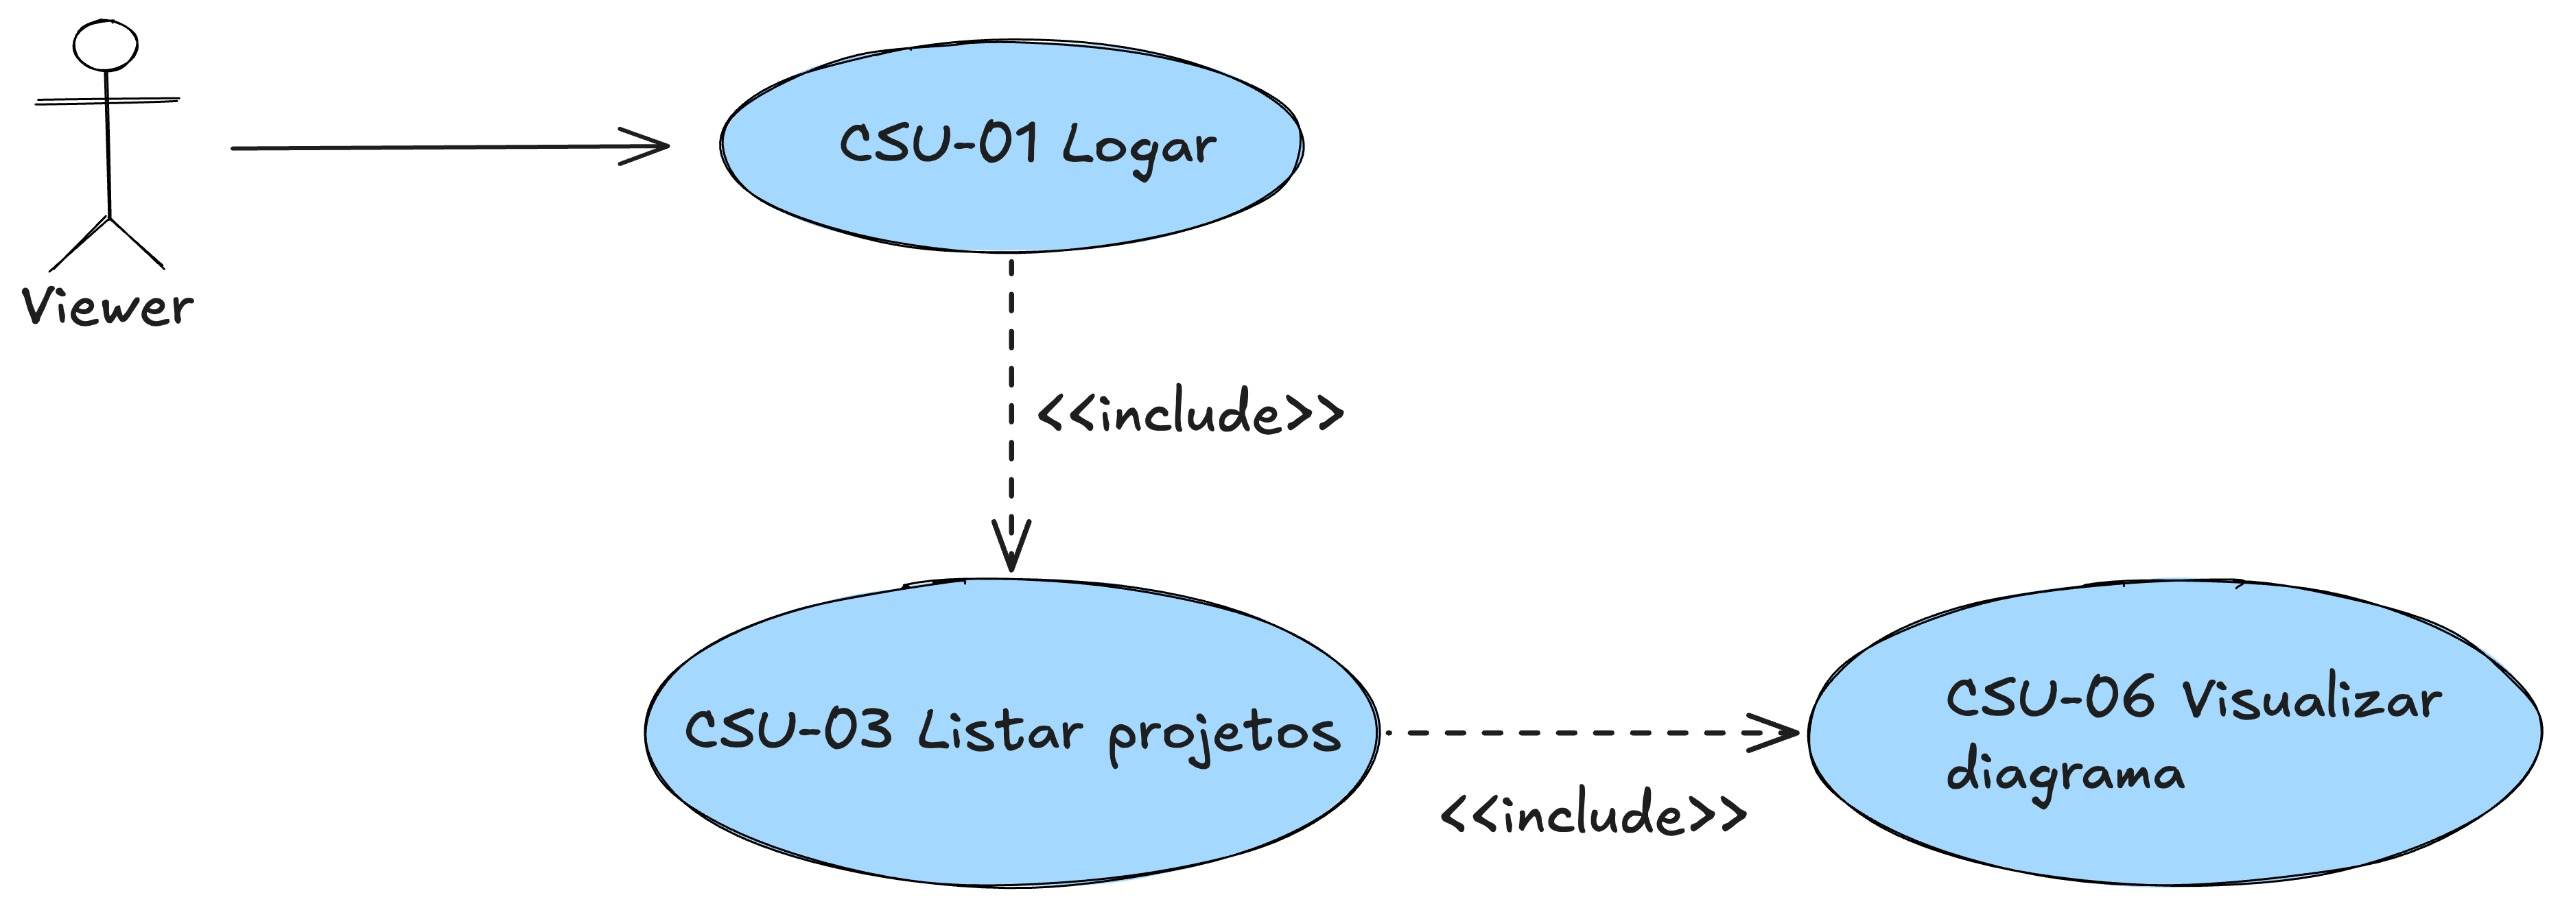
\includegraphics[scale=0.15]{figuras/viewer.jpeg}
    \caption{Diagrama de caso de uso do ator Viewer}
    \begin{center}
        {\small Fonte: Elaborado pelo autor}
    \end{center}
    \label{fig:caso-de-uso-viewer}
\end{figure}

O ator \textit{Editor}, apresentado na Figura~\ref{fig:caso-de-uso-editor}, herda as capacidades do \textit{Viewer} e adiciona a permissão de editar diagramas. Por meio dessa funcionalidade, o \textit{Editor} pode adicionar, editar e remover tabelas, gerenciar os atributos de cada tabela, criar e excluir relacionamentos entre entidades, reposicionar elementos na área de desenho, além de exportar e importar scripts SQL.

\begin{figure}[H]
    \centering
    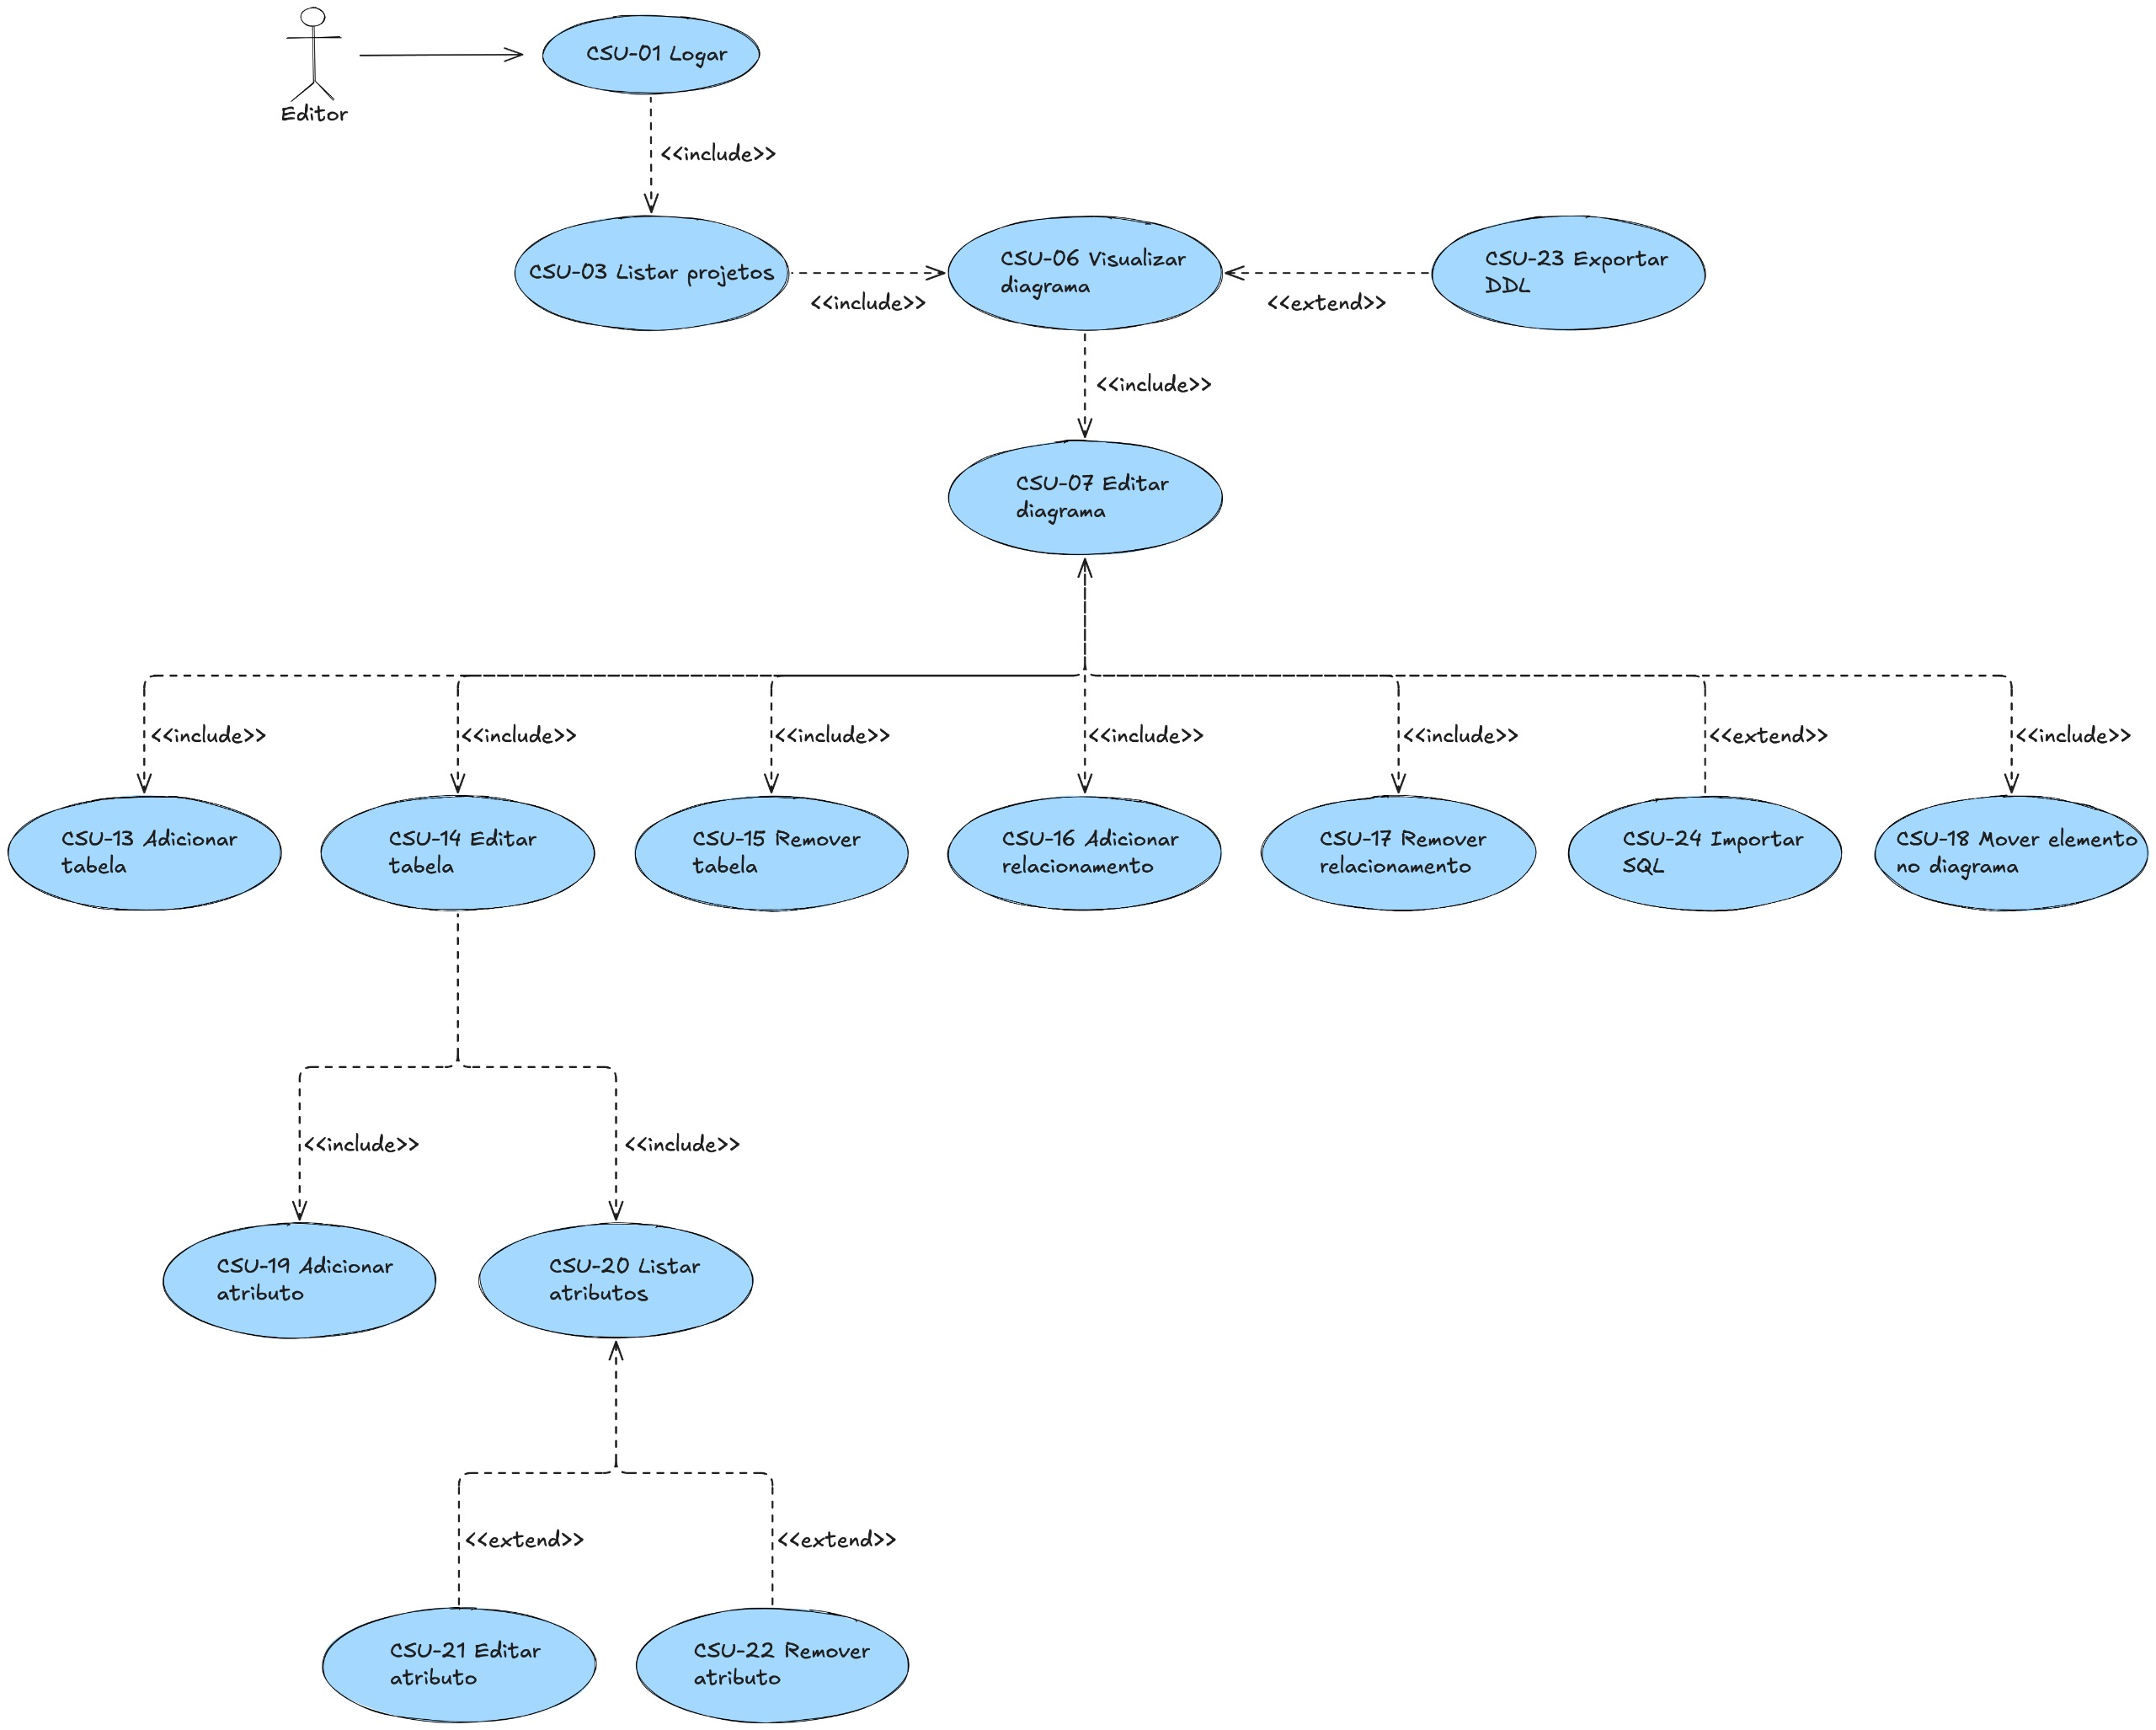
\includegraphics[scale=0.15]{figuras/editor.jpeg}
    \caption{Diagrama de caso de uso do ator Editor}
    \begin{center}
        {\small Fonte: Elaborado pelo autor}
    \end{center}
    \label{fig:caso-de-uso-editor}
\end{figure}

O ator \textit{Owner}, apresentado na Figura~\ref{fig:caso-de-uso-owner}, possui o conjunto mais amplo de permissões. Além de todas as capacidades do \textit{Editor}, o \textit{Owner} é o responsável pelo ciclo de vida dos projetos: pode criá-los, editá-los e removê-los. Também gerencia o time de colaboradores, podendo adicionar membros, listar os membros existentes, alterar seus papéis de acesso e removê-los do projeto.

\begin{figure}[H]
    \centering
    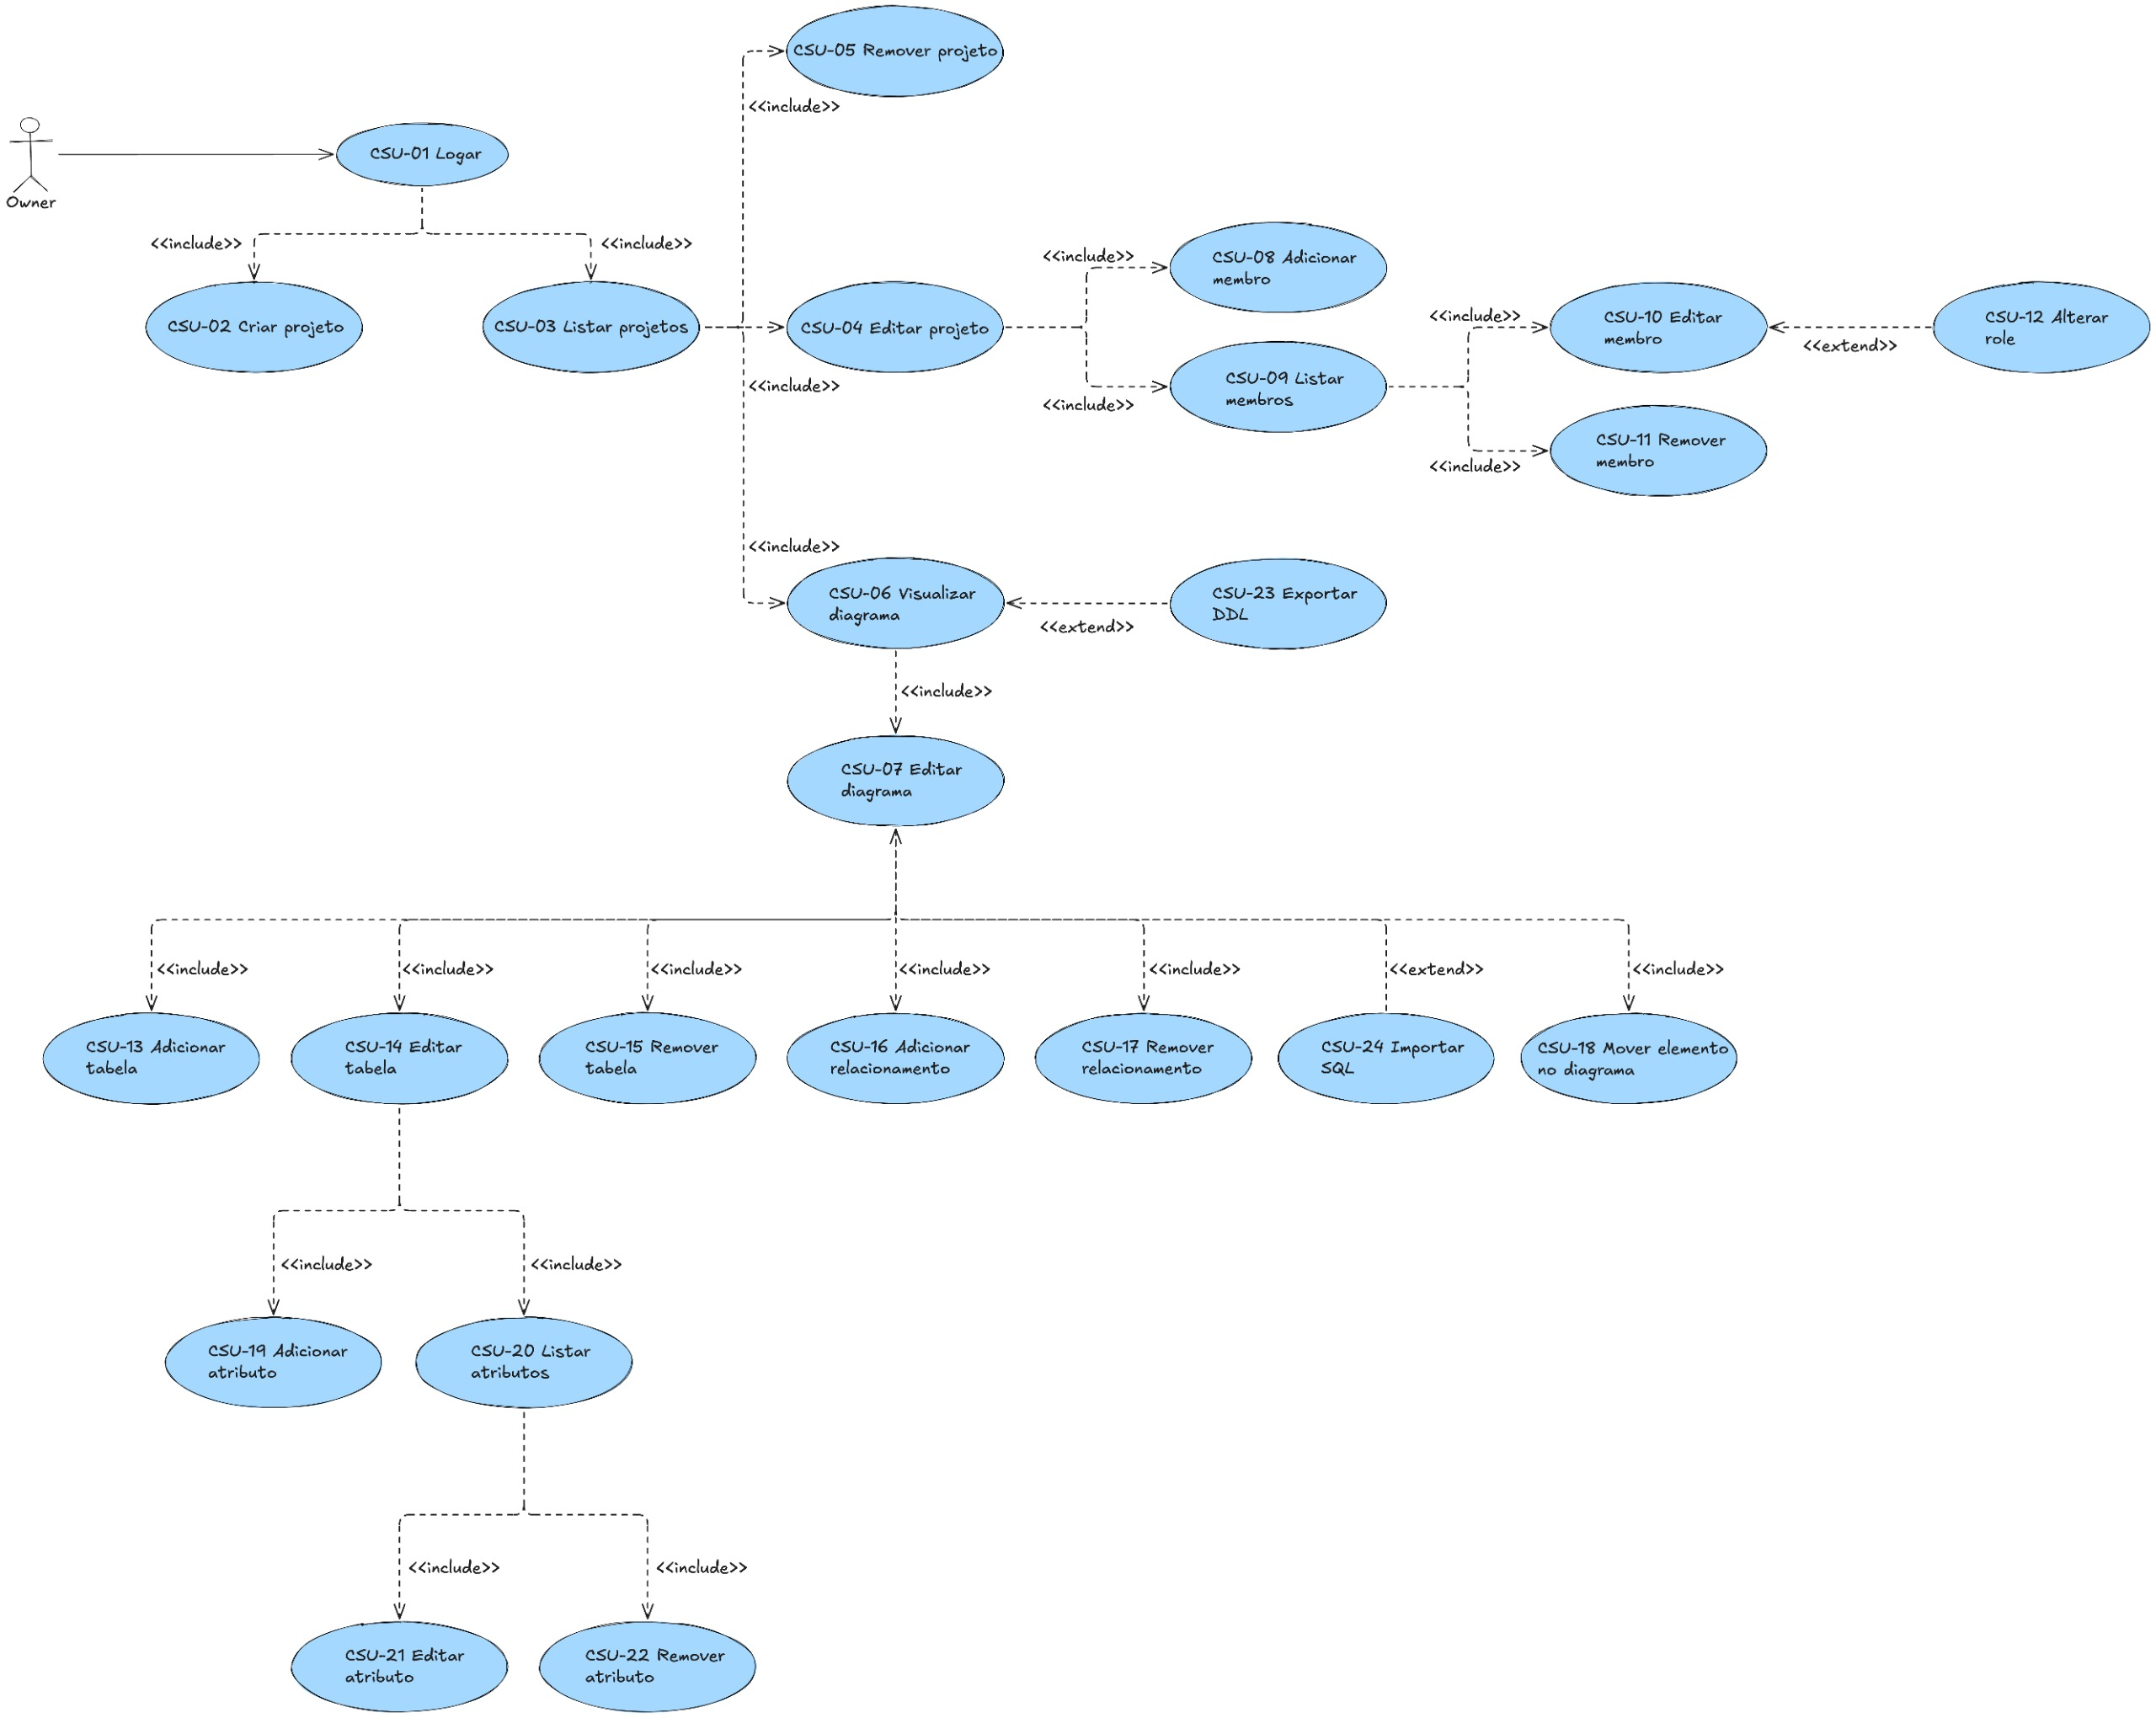
\includegraphics[scale=0.15]{figuras/owner.jpeg}
    \caption{Diagrama de caso de uso do ator Owner}
    \begin{center}
        {\small Fonte: Elaborado pelo autor}
    \end{center}
    \label{fig:caso-de-uso-owner}
\end{figure}

\section{Modelos de Dados}

As figuras \ref{fig:modelo-conceitual}, \ref{fig:modelo-logico} e \ref{fig:modelo-nosql} apresentam, respectivamente, os artefatos de modelagem de dados produzidos no projeto: o modelo conceitual e o modelo lógico do banco de dados relacional, e o esquema não-relacional com MongoDB.

O modelo conceitual define as entidades e relacionamentos de alto nível, representando a estrutura geral dos dados.

\begin{figure}[H]
    \centering
    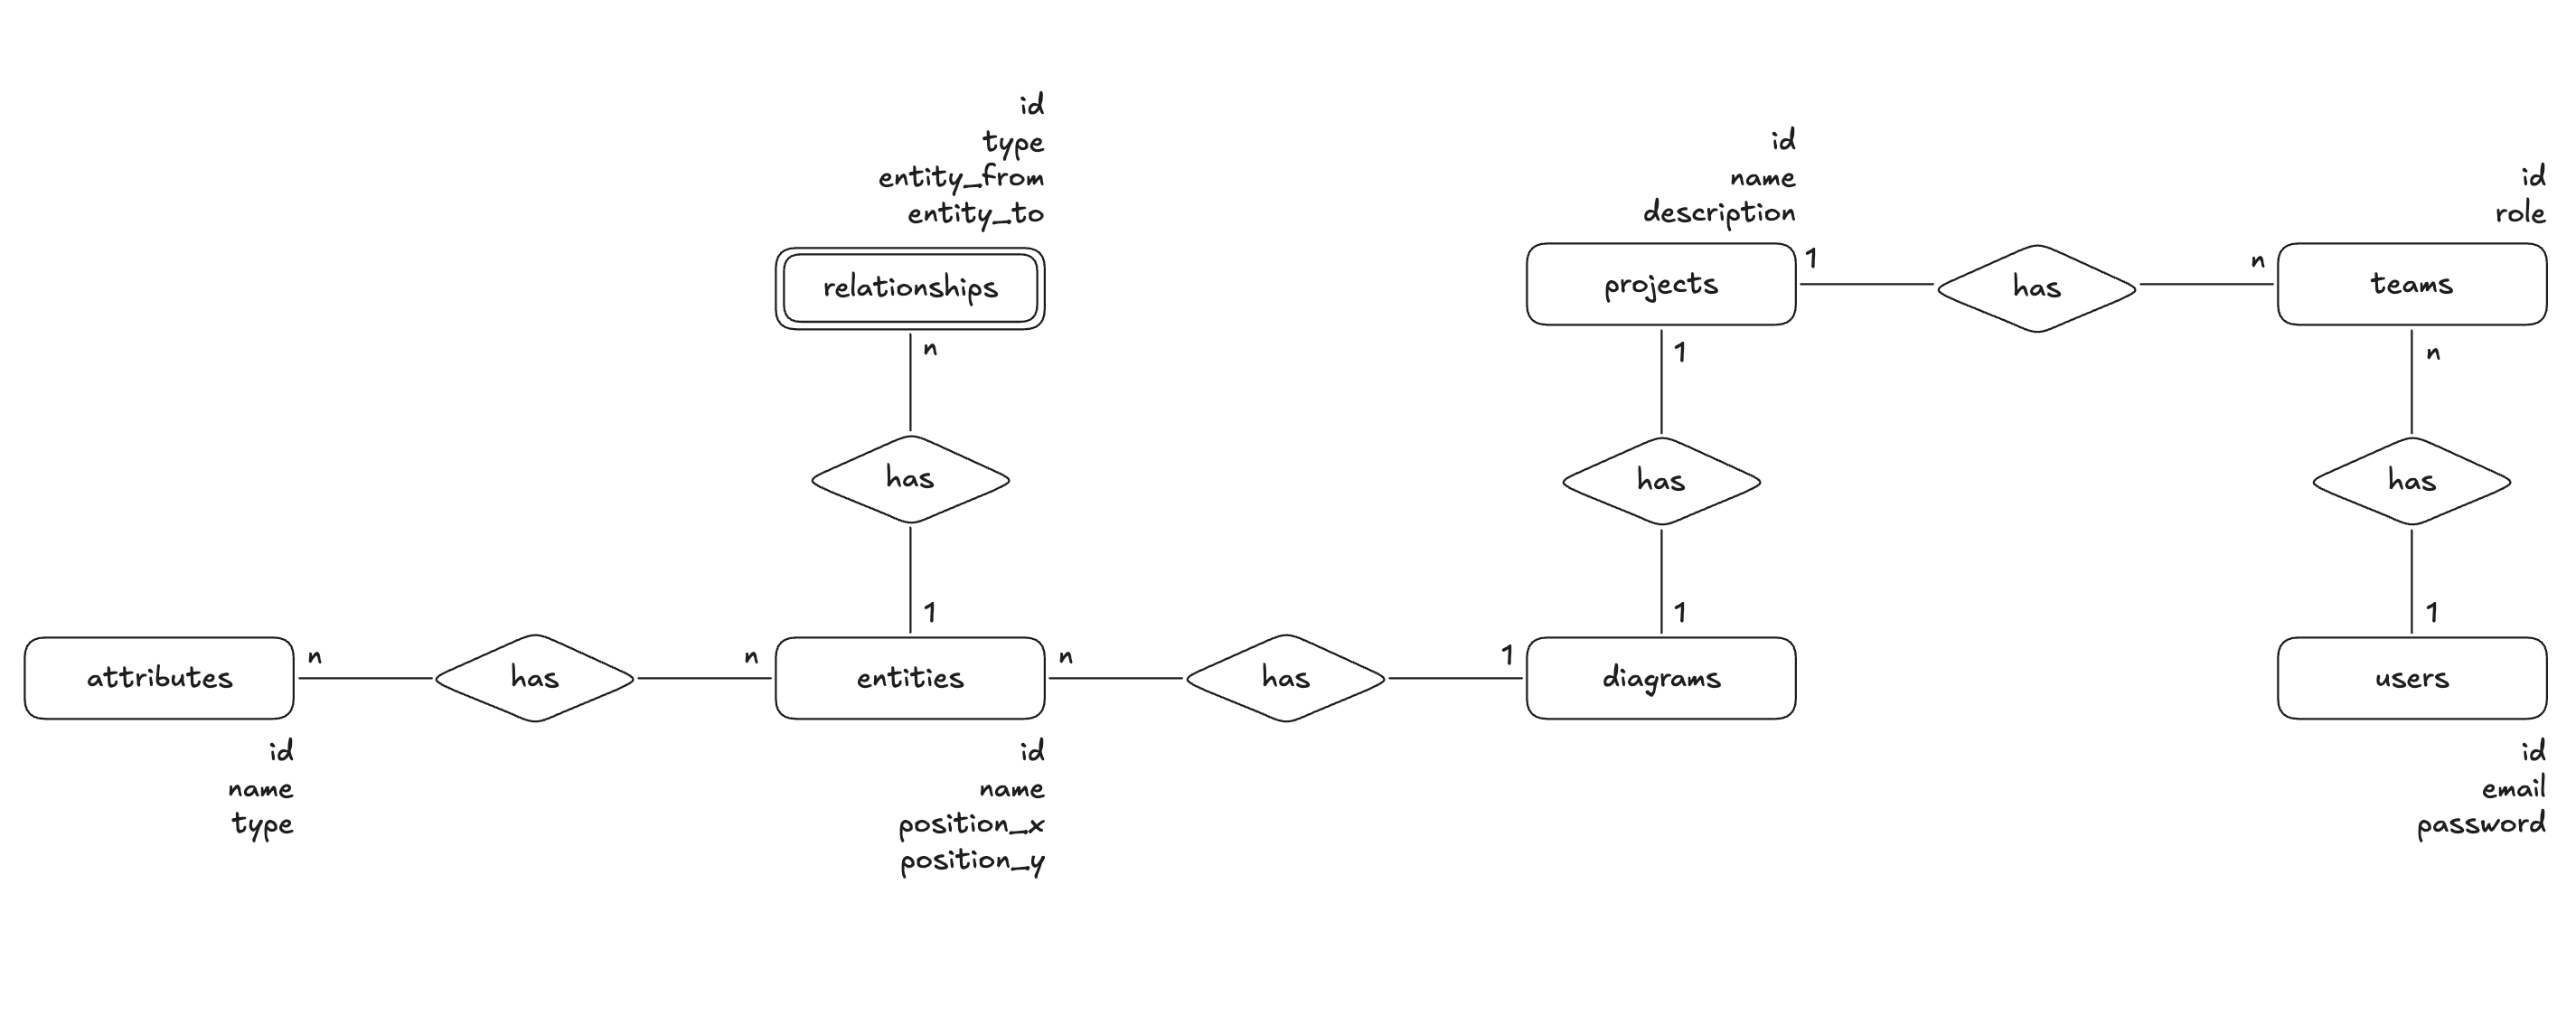
\includegraphics[width=15cm]{figuras/erd-conceptual-model.png}
    \caption{Modelo conceitual do banco de dados}
    \begin{center}
        {\small Fonte: Elaborado pelo autor}
    \end{center}
    \label{fig:modelo-conceitual}
\end{figure}

O modelo lógico detalha a estrutura das tabelas e seus atributos, considerando as características do sistema de gerenciamento de banco de dados utilizado.

\begin{figure}[H]
    \centering
    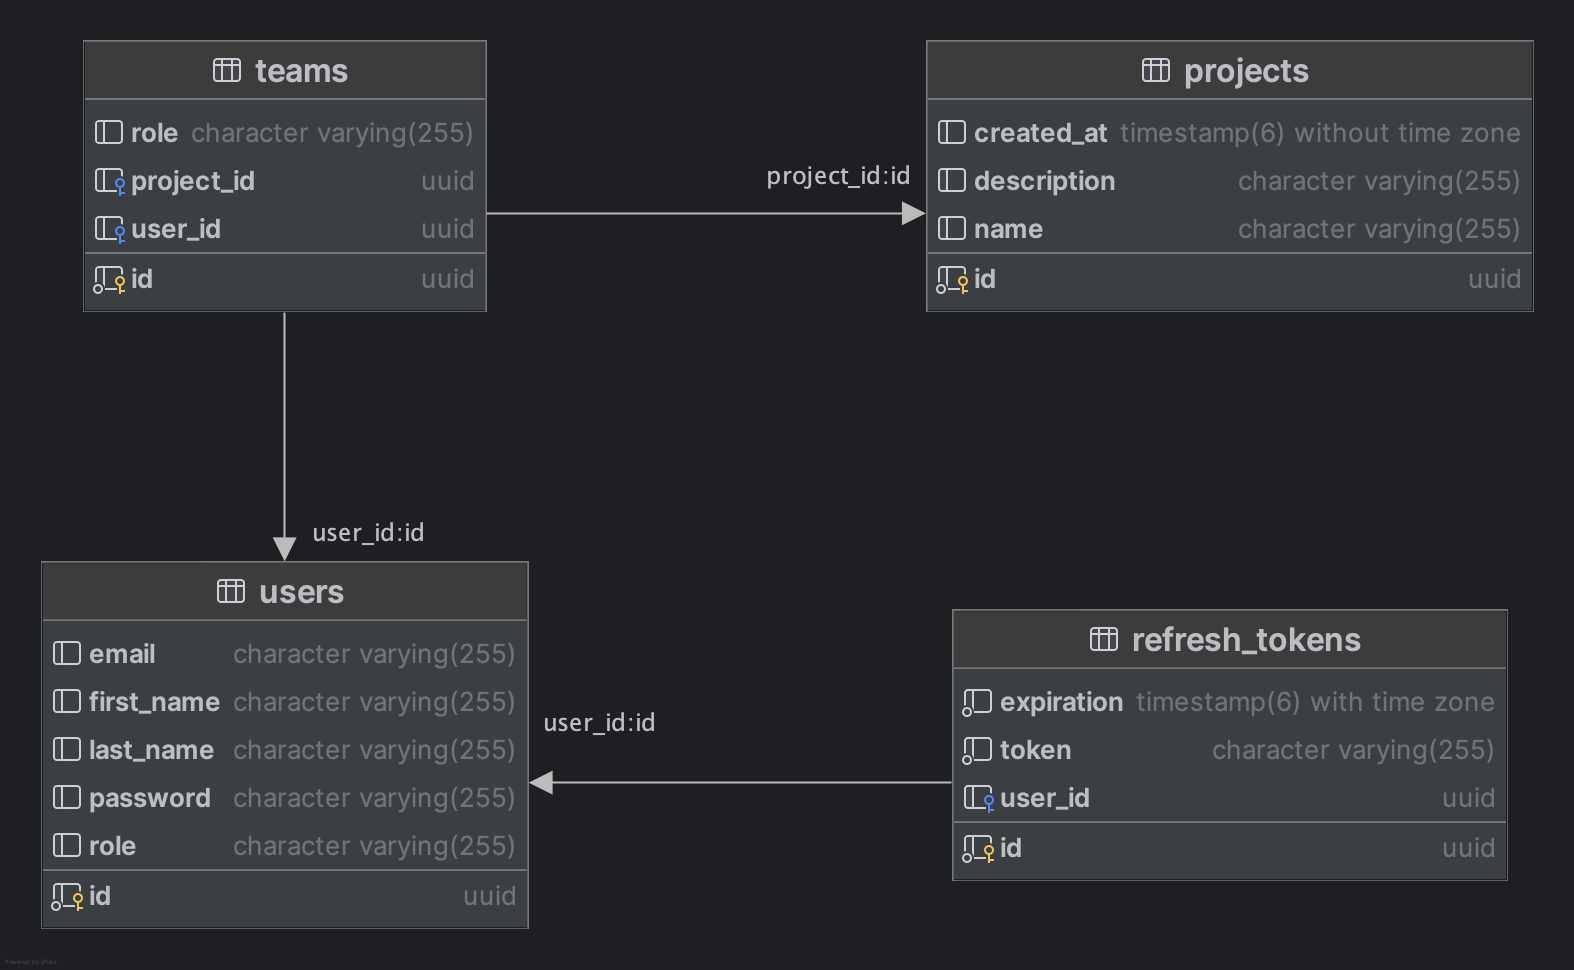
\includegraphics[width=15cm]{figuras/erd-diagram.png}
    \caption{Modelo lógico do banco de dados}
    \begin{center}
        {\small Fonte: Elaborado pelo autor}
    \end{center}
    \label{fig:modelo-logico}
\end{figure}

O esquema documental projetado para o MongoDB contempla as coleções, os campos e os tipos de dados.

\begin{figure}[H]
    \centering
    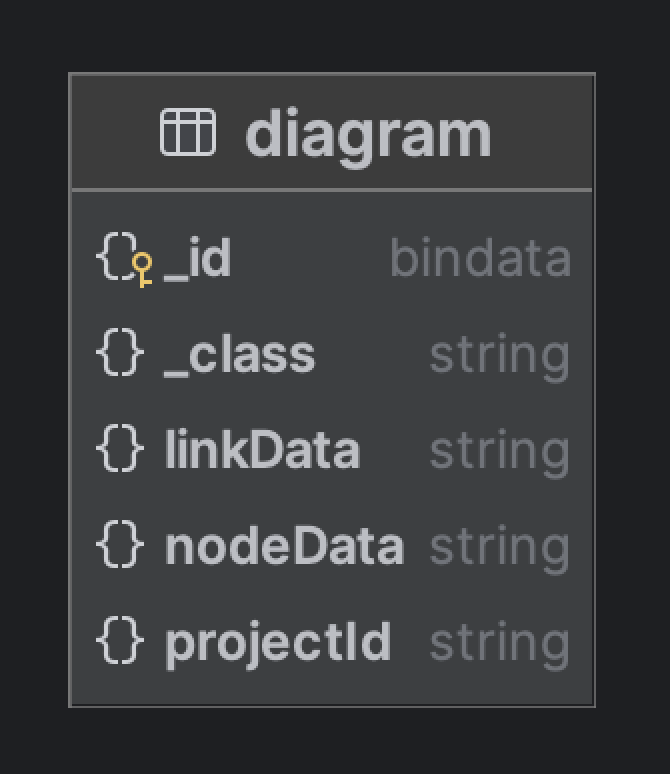
\includegraphics[width=7cm]{figuras/erd-mongodb.png}
    \caption{Esquema do banco de dados não-relacional}
    \begin{center}
        {\small Fonte: Elaborado pelo autor}
    \end{center}
    \label{fig:modelo-nosql}
\end{figure}

Os campos \textit{linkData} e \textit{nodeData} possuem, na devida ordem, os seguintes formatos:

\begin{quadro}[H]
    \begin{lstlisting}
    {
        "from": string,
        "to": string,
        "text": string,
        "toText": interger,
        "fromColumn": string      
    }
    \end{lstlisting}
    \caption{Estrutura de dados do campo \textit{linkData}}
    \begin{center}
        {\small Fonte: Elaborado pelo autor}
    \end{center}
    \label{lst:link-data}
\end{quadro}

\begin{quadro}[H]
    \begin{lstlisting}
    {
        "id": string,
        "key": string,
        "items": [
            {
            "name": string,
            "type": string,
            "pk": boolean,
            "fk": boolean,
            "unique": boolean,
            "notNull": boolean,
            "autoIncrement": boolean,
            "defaultValue": string
            }
        ],
        "location": {
            "x": string,
            "y": string
        }
    }
    \end{lstlisting}
    \caption{Estrutura de dados do campo \textit{nodeData}}
    \begin{center}
        {\small Fonte: Elaborado pelo autor}
    \end{center}
    \label{lst:node-data}
\end{quadro}

\section{Arquitetura do Protótipo}

O protótipo foi construído segundo a arquitetura cliente-servidor, composta por dois módulos independentes: o \textit{back-end}, implementado com Spring Boot, e o \textit{front-end}, desenvolvido com Angular. A Figura~\ref{fig:arquitetura} apresenta uma visão geral dos componentes do sistema e dos canais de comunicação entre eles.

\begin{figure}[H]
    \centering
    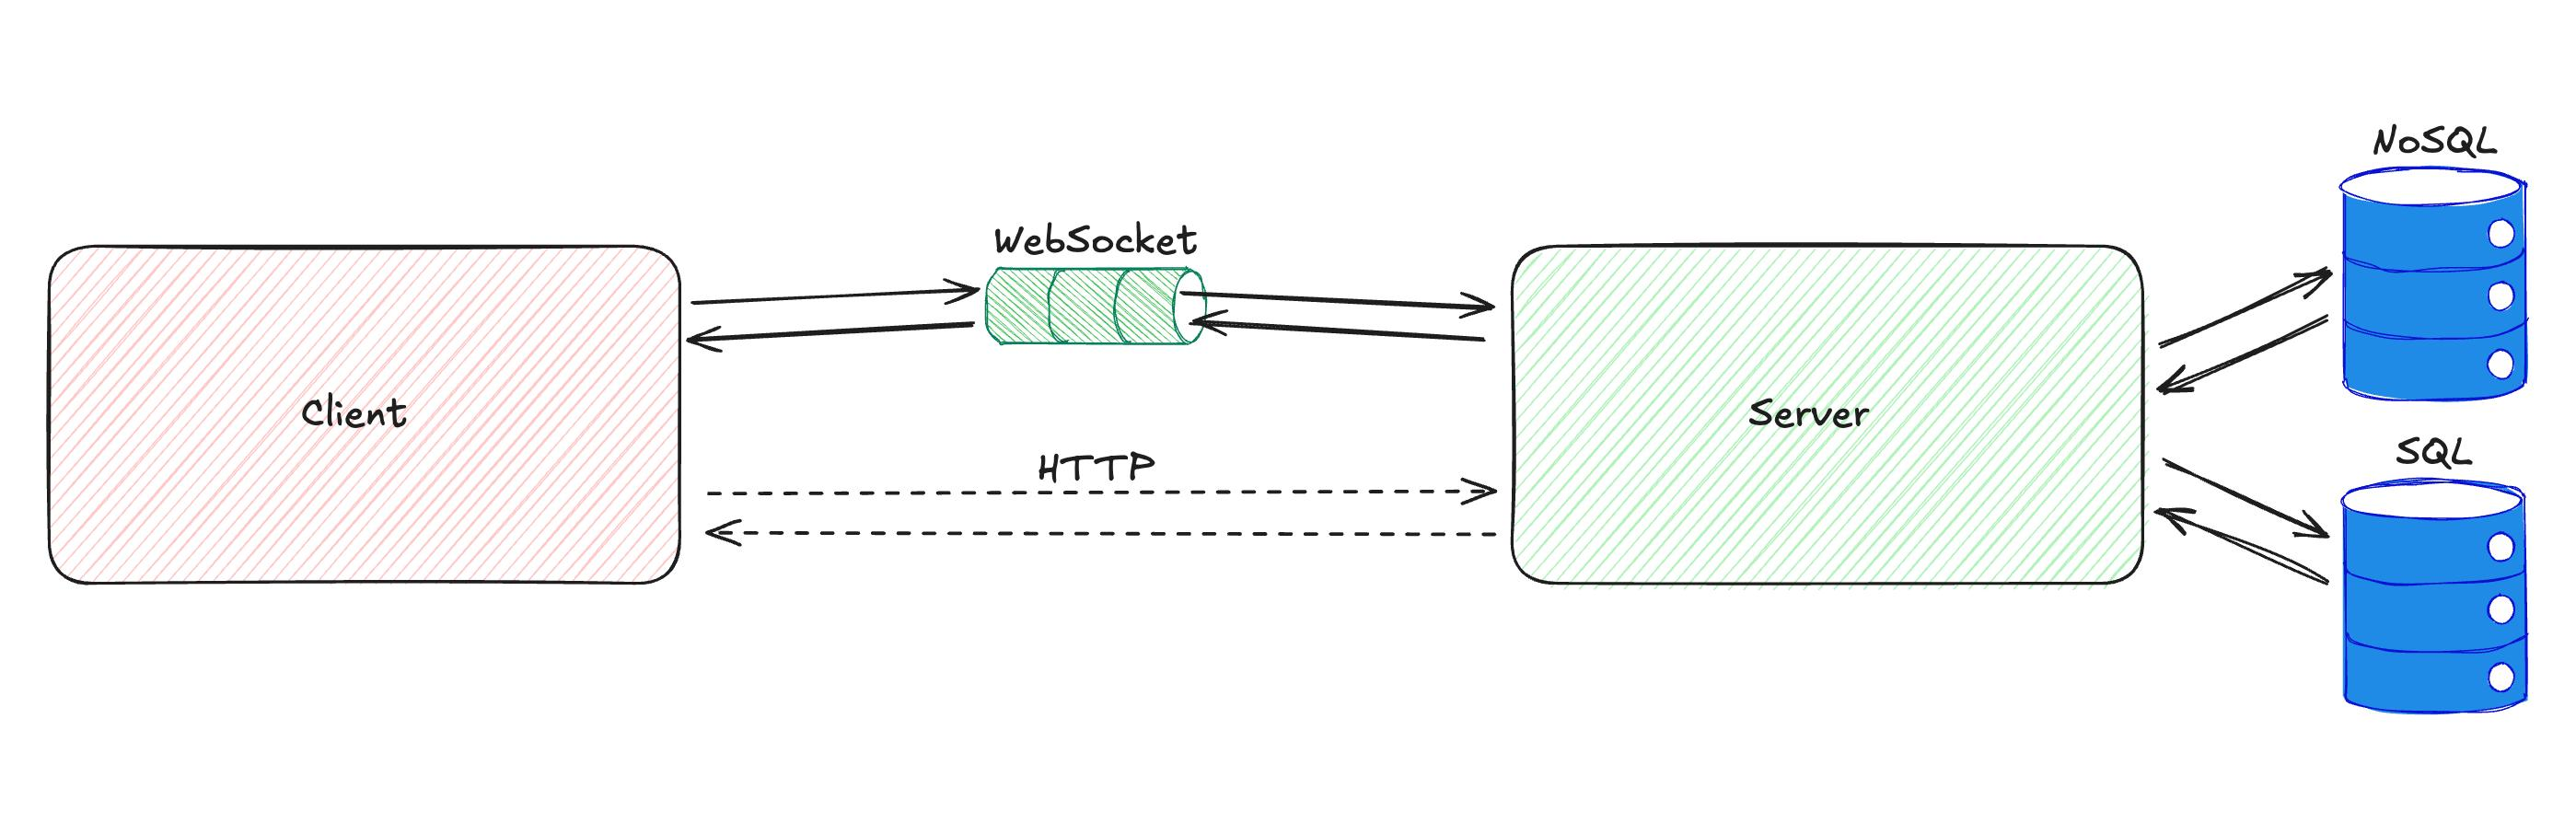
\includegraphics[width=15cm]{figuras/desenho-da-arquitetura.jpeg}
    \caption{Arquitetura do protótipo}
    \begin{center}
        {\small Fonte: Elaborado pelo autor}
    \end{center}
    \label{fig:arquitetura}
\end{figure}

A comunicação entre os módulos ocorre por dois canais distintos: requisições HTTP para as operações de persistência e autenticação, e uma conexão persistente via WebSocket para a sincronização colaborativa em tempo real.

O \textit{back-end} foi organizado em camadas seguindo o padrão MVC, separando as responsabilidades de controle, regras de negócio e acesso a dados. A segurança da API é gerenciada por meio de \textit{tokens} JWT armazenados em \textit{cookies} no navegador do cliente, protegendo os recursos contra acesso não autorizado. A comunicação em tempo real é viabilizada por um servidor WebSocket dedicado, responsável por receber as ações dos colaboradores e propagá-las a todos os usuários conectados ao mesmo projeto.

O \textit{front-end} é estruturado como uma SPA, com responsabilidades distribuídas entre componentes de interface, serviços de dados e interceptadores de requisição. O componente central do editor integra a biblioteca GoJS para a renderização e manipulação interativa do diagrama no \textit{canvas}, enquanto serviços dedicados encapsulam a comunicação em tempo real e as operações de importação e exportação SQL.

\section{Funcionalidades Implementadas}

As subseções a seguir descrevem as funcionalidades que compõem o protótipo desenvolvido.

\subsection{Autenticação e Autorização}

O protótipo implementa um fluxo de autenticação com credenciais de acesso. Após a autenticação bem-sucedida, o servidor emite dois \textit{tokens} de segurança: um de curta duração para as requisições e outro de renovação, ambos armazenados de forma segura no navegador do cliente. As rotas da aplicação são protegidas tanto no lado do cliente quanto no servidor, garantindo que apenas usuários autenticados acessem os recursos. Quando o \textit{token} de acesso expira, a renovação ocorre de forma automática e transparente ao usuário, sem necessidade de novo \textit{login}.

A Figura~\ref{fig:arquitetura-autenticacao} ilustra a arquitetura de autenticação e autorização implementada no \textit{back-end}. Toda requisição originada pelo cliente passa pelo filtro JWT, que valida o \textit{token} presente no \textit{cookie}; caso inválido, a requisição é rejeitada com o código 401 (\textit{Unauthorized}). Requisições válidas avançam para duas camadas de autorização em série: a primeira verifica permissões com base na URL acessada e a segunda aplica restrições mais granulares ao nível do método, controlando o acesso de acordo com o perfil do usuário autenticado. O descumprimento de qualquer uma dessas camadas resulta em resposta 403 (\textit{Forbidden}); somente após a aprovação em ambas a requisição alcança os controladores da aplicação.

\begin{figure}[H]
    \centering
    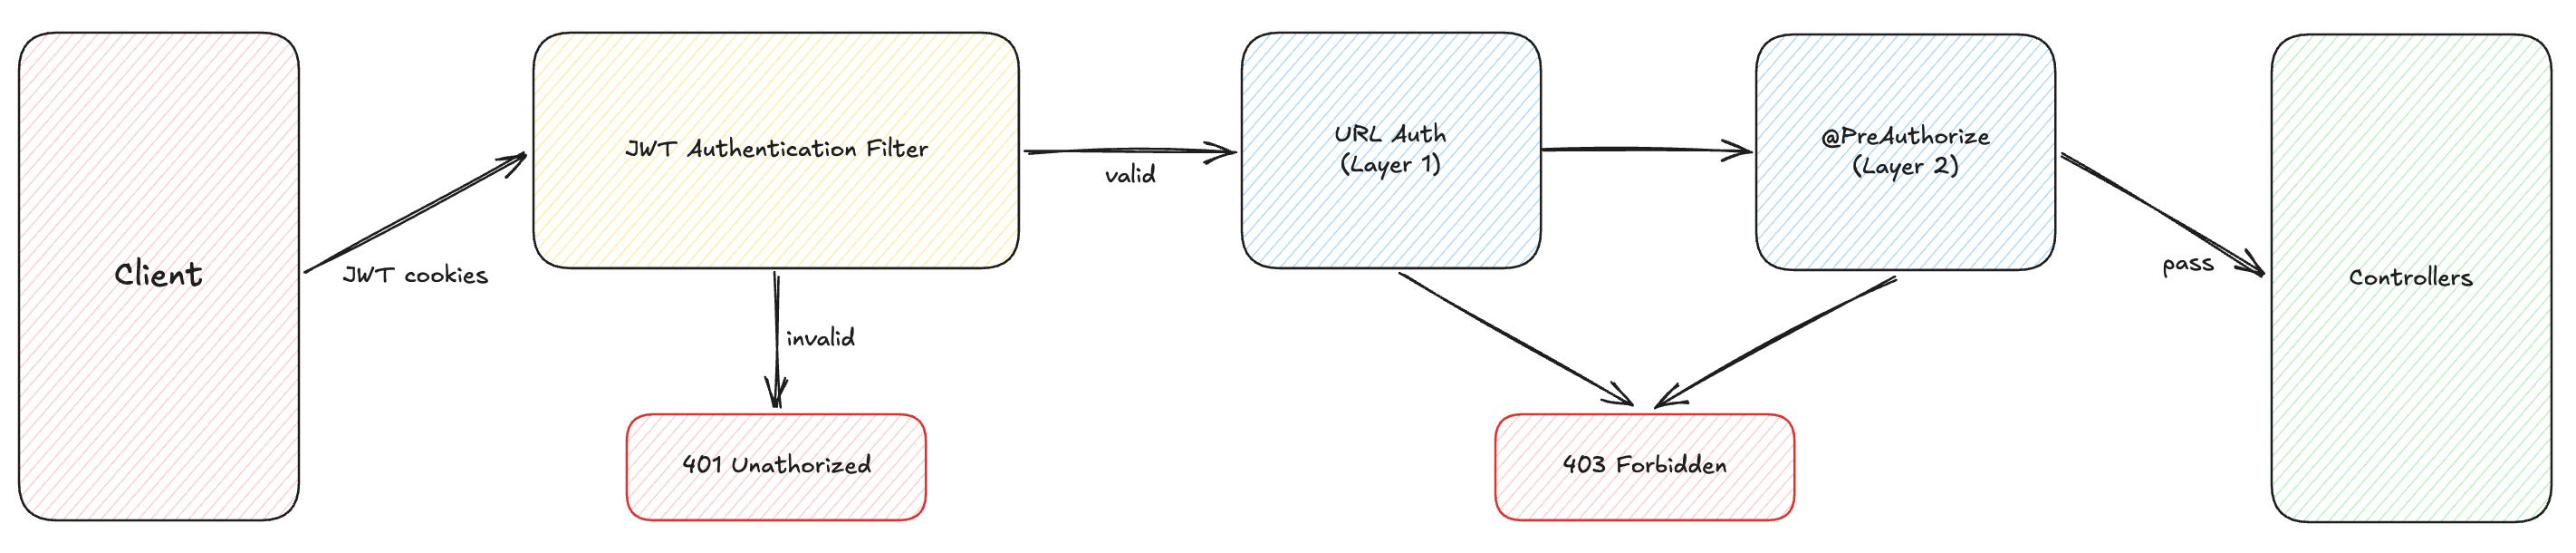
\includegraphics[width=\textwidth]{figuras/desenho-da-arquitetura-de-autenticacao-e-autorizacao.jpeg}
    \caption{Arquitetura de autenticação e autorização do \textit{back-end}}
    \begin{center}
        {\small Fonte: Elaborado pelo autor}
    \end{center}
    \label{fig:arquitetura-autenticacao}
\end{figure}

\subsection{Gerenciamento de Projetos e Times}

O sistema permite ao usuário criar e gerenciar projetos de modelagem. Cada projeto possui um time de colaboradores, para o qual o criador pode convidar outros usuários cadastrados na plataforma. A gestão de projetos e times é realizada por meio de uma interface de \textit{dashboard}, com operações de criação, leitura, atualização e exclusão comunicadas ao servidor e persistidas no banco de dados.

\subsection{Editor de Diagramas ER}

O editor de diagramas constitui o componente central do protótipo. Construído com a biblioteca GoJS, o \textit{canvas} permite adicionar e remover entidades (tabelas), gerenciar seus atributos com configuração de tipo de dado, chave primária, chave estrangeira, unicidade, restrição não nulo, auto-incremento e valor padrão, criar e excluir relacionamentos entre entidades com definição de cardinalidade, além de reposicionar livremente os elementos na área de desenho. O estado completo do diagrama (entidades, atributos, relacionamentos e posicionamentos) é persistido na base de dados ao final de cada sequência de ações.

\subsection{Colaboração em Tempo Real}

A funcionalidade de colaboração permite que múltiplos usuários de um mesmo time trabalhem simultaneamente no mesmo diagrama. Ao abrir um projeto, o cliente estabelece automaticamente uma conexão persistente com o servidor para receber atualizações em tempo real. Quando um usuário seleciona uma entidade para edição, uma notificação de bloqueio é imediatamente propagada a todos os demais colaboradores conectados. Enquanto o bloqueio está ativo, a entidade correspondente fica indisponível para edição pelos outros usuários, prevenindo conflitos de concorrência. O bloqueio é liberado automaticamente pelo servidor após um intervalo de tempo predefinido, caso o usuário não o libere explicitamente.

\subsection{Importação e Exportação de Diagramas}

O protótipo suporta a interoperabilidade com outros ambientes por meio de operações SQL no dialeto MySQL. A exportação converte o modelo do diagrama em instruções SQL de criação de tabelas, enquanto a importação analisa um \textit{script} SQL fornecido pelo usuário para reconstruir o diagrama correspondente no \textit{canvas}. Ambas as operações são processadas pelo \textit{back-end} e o resultado é retornado ao usuário pela interface da aplicação.

\section{\textit{Interface} do Usuário}

Esta seção apresenta as telas que compõem a \textit{interface} do protótipo, organizadas pelo fluxo de uso da aplicação.

% ----------------------------------------------------------
\subsection{Autenticação}
% ----------------------------------------------------------

A Figura~\ref{fig:tela-login} apresenta a tela de entrada da aplicação. O usuário informa seu \textit{e-mail} e senha para autenticar-se, com a opção de manter a sessão ativa. O cadastro de novos usuários não está disponível pela interface gráfica, sendo realizado exclusivamente por meio da API do \textit{back-end}. O Quadro~\ref{lst:curl-cadastro} apresenta o comando utilizado para esse cadastro.

\begin{figure}[H]
    \centering
    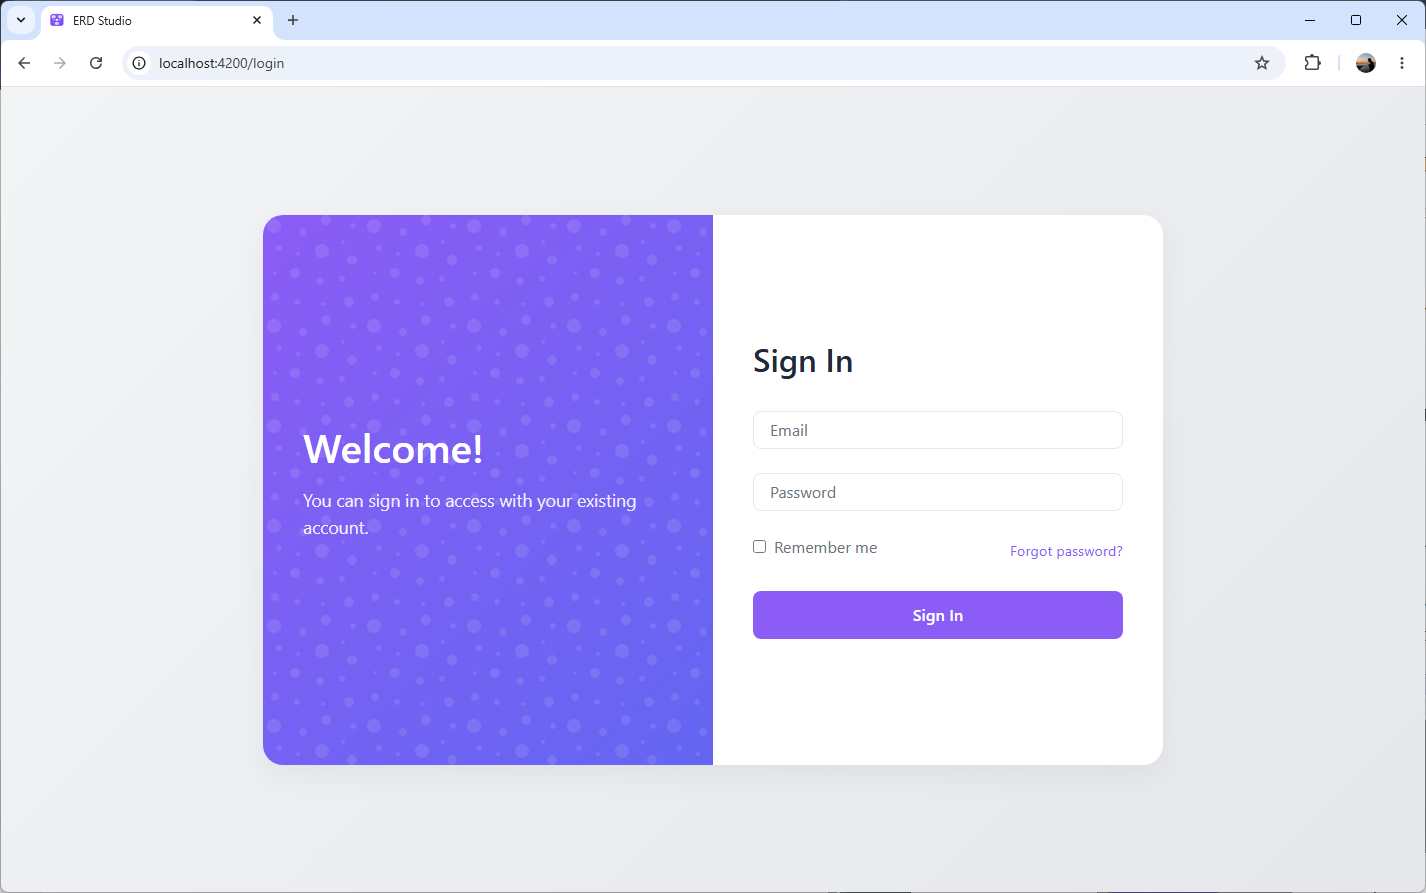
\includegraphics[width=15cm]{figuras/interface/tela-de-login.png}
    \caption{Tela de \textit{login}}
    \begin{center}
        {\small Fonte: Elaborado pelo autor}
    \end{center}
    \label{fig:tela-login}
\end{figure}

\begin{quadro}[H]
    \begin{lstlisting}
curl -X POST http://localhost:8080/api/user \
    -H "Content-Type: application/json" \
    -d '{
      "firstName": "Test",
      "lastName": "Name",
      "email": "test.name@email.com",
      "password": "yourPassword123!",
      "role": "USER"
    }'
    \end{lstlisting}
    \caption{Comando para cadastro de usuário via API}
    \begin{center}
        {\small Fonte: Elaborado pelo autor}
    \end{center}
    \label{lst:curl-cadastro}
\end{quadro}

% ----------------------------------------------------------
\subsection{Gerenciamento de Projetos e Times}
% ----------------------------------------------------------

Após o \textit{login}, o usuário é direcionado à tela principal da aplicação, apresentada na Figura~\ref{fig:tela-principal}. O menu lateral lista os projetos dos quais o usuário faz parte e disponibiliza o botão para criação de um novo projeto. Na parte inferior do menu, são exibidas as informações do usuário autenticado e a opção de encerrar a sessão.

\begin{figure}[H]
    \centering
    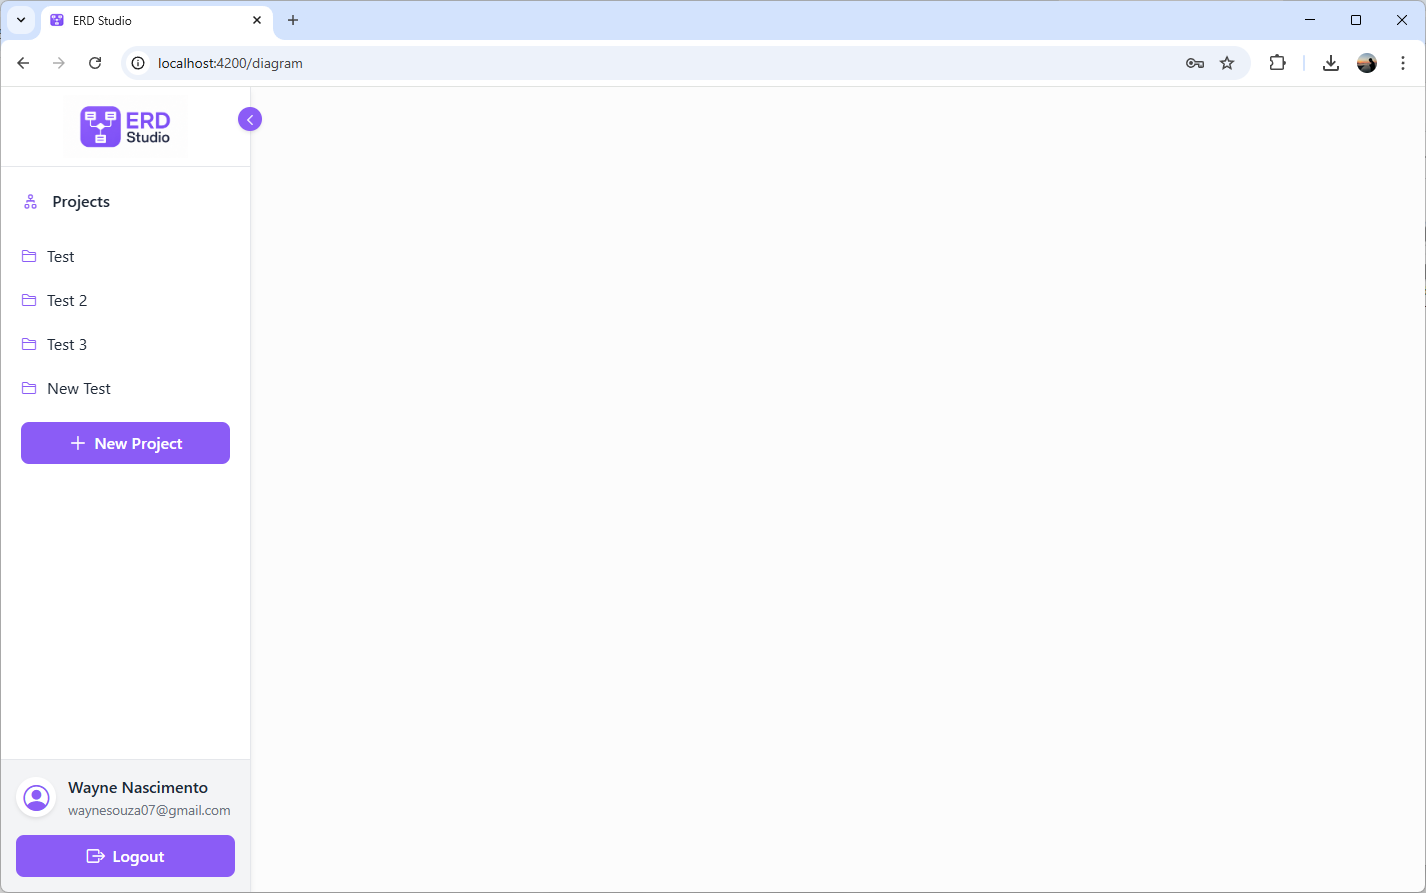
\includegraphics[width=15cm]{figuras/interface/tela-principal.png}
    \caption{Tela principal com listagem de projetos}
    \begin{center}
        {\small Fonte: Elaborado pelo autor}
    \end{center}
    \label{fig:tela-principal}
\end{figure}

Ao acionar o botão de criação, é exibido o \textit{modal} apresentado na Figura~\ref{fig:criacao-projeto}. O usuário informa o nome e a descrição do projeto e confirma a operação. O projeto criado passa a aparecer imediatamente no menu lateral.

\begin{figure}[H]
    \centering
    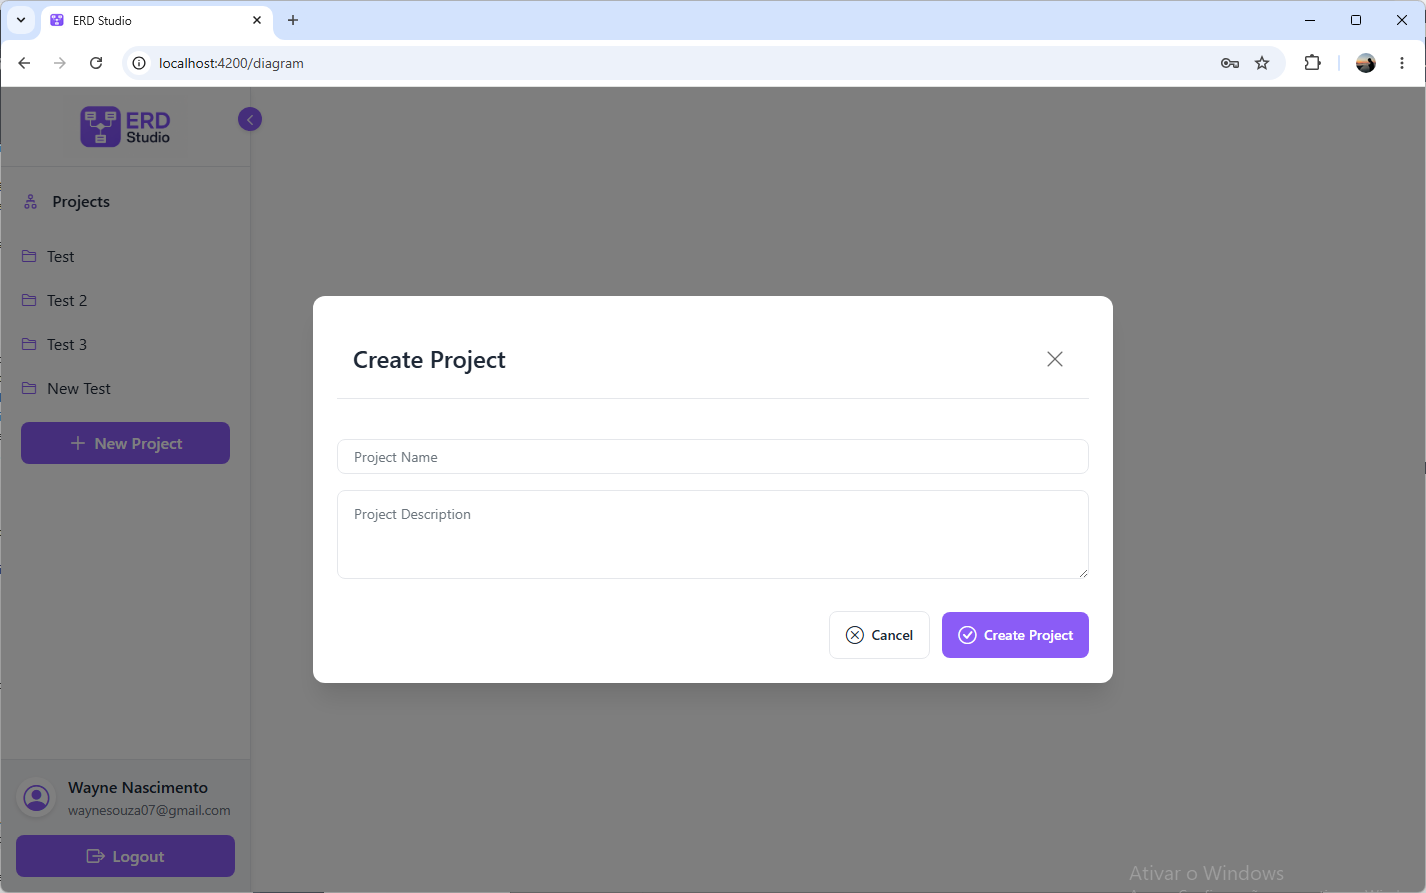
\includegraphics[width=15cm]{figuras/interface/modal-de-criacao-de-projeto.png}
    \caption{\textit{Modal} de criação de projeto}
    \begin{center}
        {\small Fonte: Elaborado pelo autor}
    \end{center}
    \label{fig:criacao-projeto}
\end{figure}

A Figura~\ref{fig:edicao-projeto} ilustra o \textit{modal} de edição de projeto, que reúne em uma única tela a edição dos dados do projeto e o gerenciamento do time de colaboradores. A seção \textit{Team Members} lista os membros com seus respectivos papéis de acesso, e o \textit{Owner} pode adicionar ou remover colaboradores e alterar seus papéis. A tela também disponibiliza a opção de excluir o projeto.

\begin{figure}[H]
    \centering
    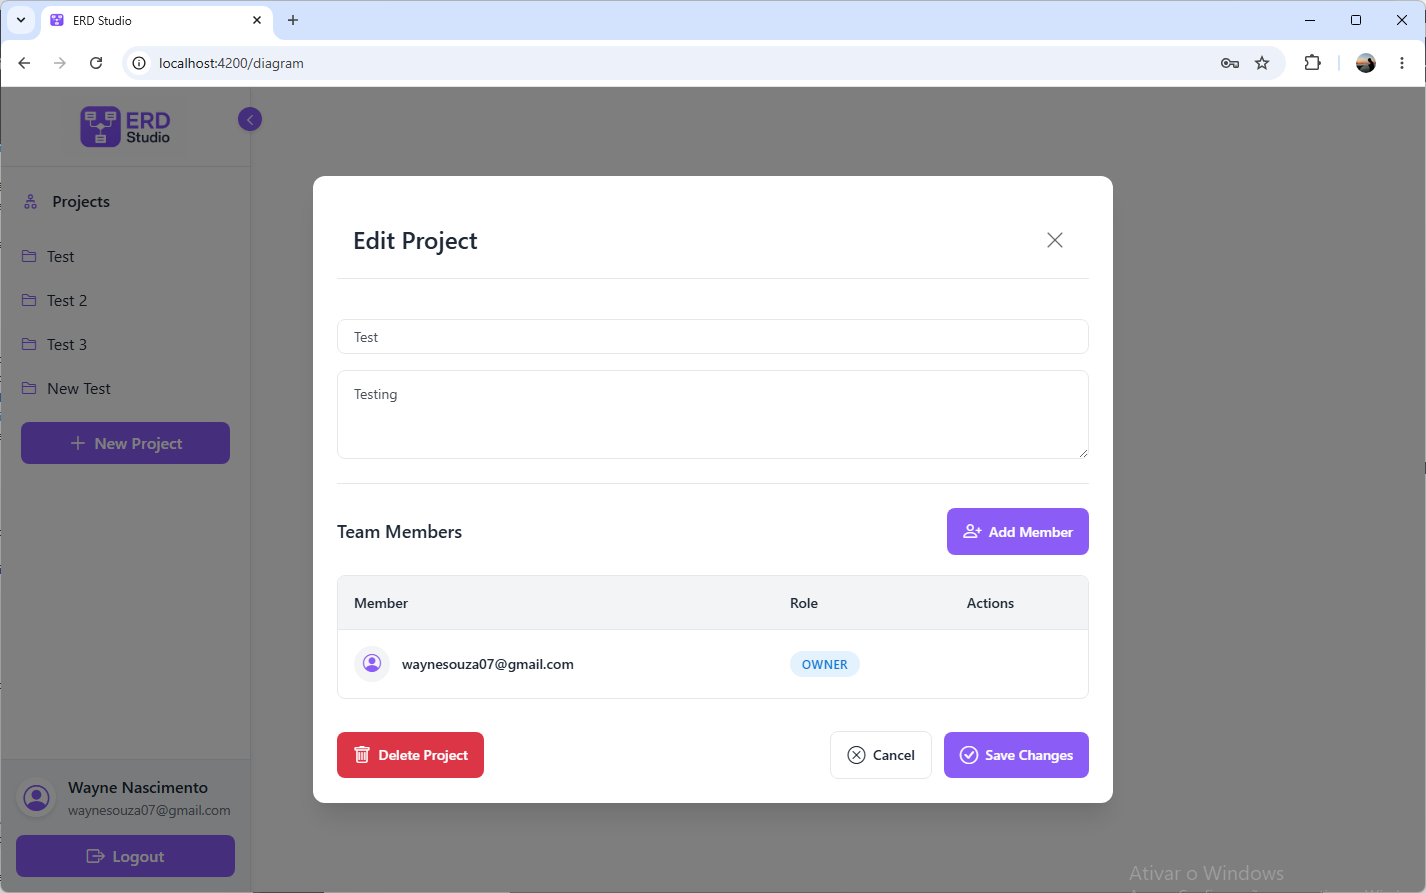
\includegraphics[width=15cm]{figuras/interface/modal-de-edicao-de-projeto.png}
    \caption{\textit{Modal} de edição de projeto e gerenciamento de time}
    \begin{center}
        {\small Fonte: Elaborado pelo autor}
    \end{center}
    \label{fig:edicao-projeto}
\end{figure}

A adição de um novo membro é realizada por meio de um \textit{modal} secundário, apresentado na Figura~\ref{fig:adicionar-membro}. O \textit{Owner} informa o e-mail do colaborador e seleciona o papel de acesso a ser atribuído (\textit{Viewer} ou \textit{Editor}).

\begin{figure}[H]
    \centering
    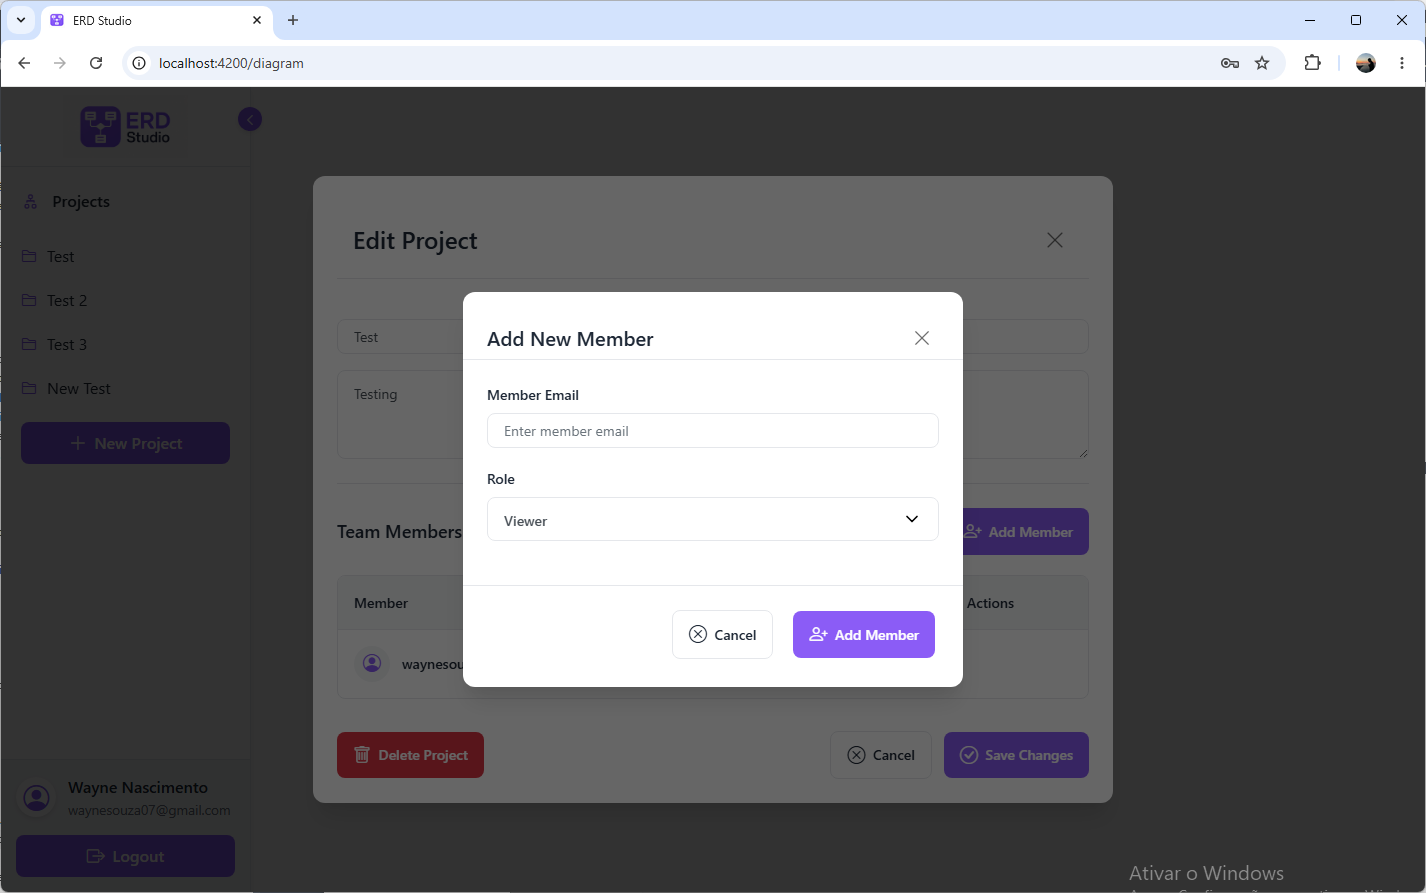
\includegraphics[width=15cm]{figuras/interface/modal-de-adicao-de-membro-no-projeto.png}
    \caption{\textit{Modal} de adição de membro ao projeto}
    \begin{center}
        {\small Fonte: Elaborado pelo autor}
    \end{center}
    \label{fig:adicionar-membro}
\end{figure}

% ----------------------------------------------------------
\subsection{Editor de Diagramas}
% ----------------------------------------------------------

Ao selecionar um projeto no menu lateral, o usuário acessa o editor de diagramas. A Figura~\ref{fig:diagrama-vazio} apresenta o editor com um diagrama composto por três entidades e seus respectivos relacionamentos. A barra de ferramentas lateral disponibiliza as ações de modelagem: adição de entidade, definição do tipo de relacionamento e operações de importação e exportação SQL. No topo da tela, o papel do usuário no projeto é exibido em destaque.

\begin{figure}[H]
    \centering
    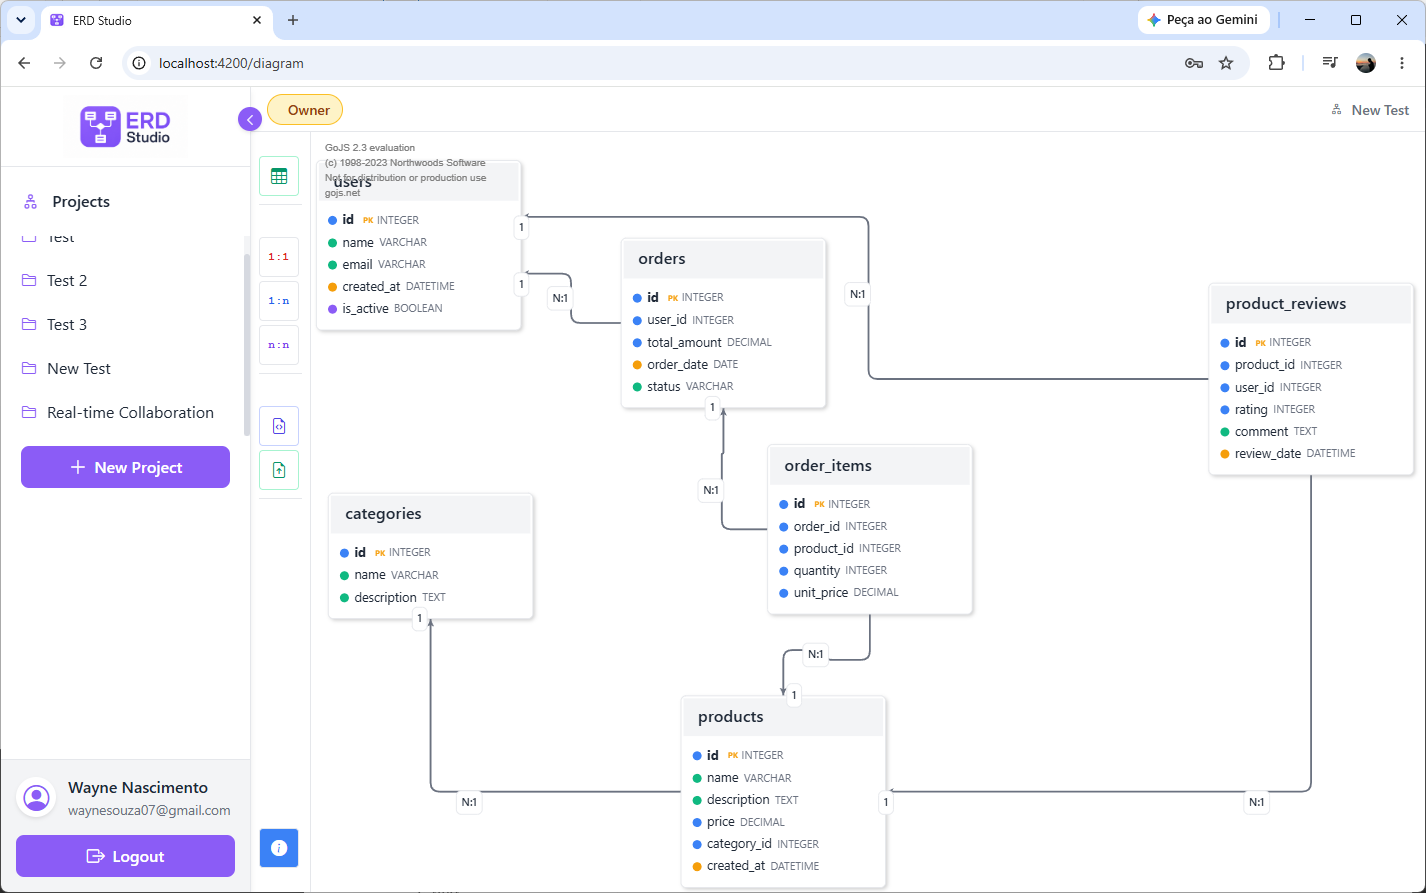
\includegraphics[width=15cm]{figuras/interface/tela-com-diagrama-simples.png}
    \caption{Editor de diagramas com entidades e relacionamentos}
    \begin{center}
        {\small Fonte: Elaborado pelo autor}
    \end{center}
    \label{fig:diagrama-vazio}
\end{figure}

Ao adicionar ou selecionar uma entidade no \textit{canvas}, o \textit{modal} de edição apresentado na Figura~\ref{fig:edicao-entidade} é exibido. O usuário define o nome da entidade e gerencia seus atributos por meio de uma tabela interativa. Para cada atributo, é possível configurar o nome, o tipo de dado e as restrições aplicáveis: chave primária, unicidade, obrigatoriedade, auto-incremento e valor padrão. Novos atributos são adicionados por meio do botão disponível no rodapé do \textit{modal}.

\begin{figure}[H]
    \centering
    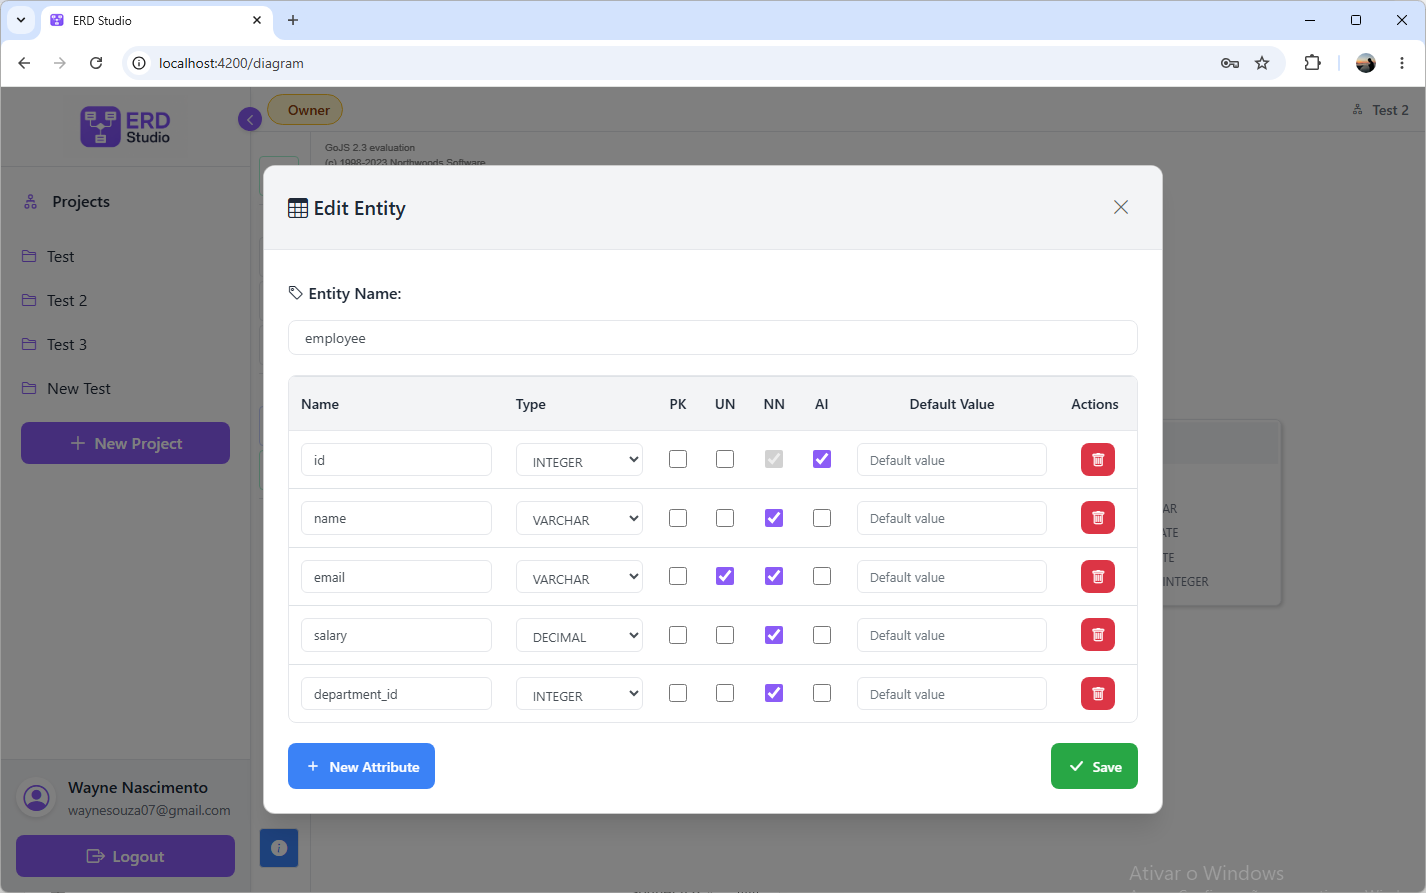
\includegraphics[width=15cm]{figuras/interface/modal-de-edicao-da-tabela.png}
    \caption{\textit{Modal} de edição de entidade}
    \begin{center}
        {\small Fonte: Elaborado pelo autor}
    \end{center}
    \label{fig:edicao-entidade}
\end{figure}

A Figura~\ref{fig:diagrama-com-entidades} exibe o mesmo diagrama com a legenda visível no \textit{canvas}. A legenda descreve o código de cores utilizado para representar os tipos de dados dos atributos e indica os marcadores de chave primária. O diagrama reflete em tempo real as alterações realizadas por qualquer colaborador conectado ao projeto.

\begin{figure}[H]
    \centering
    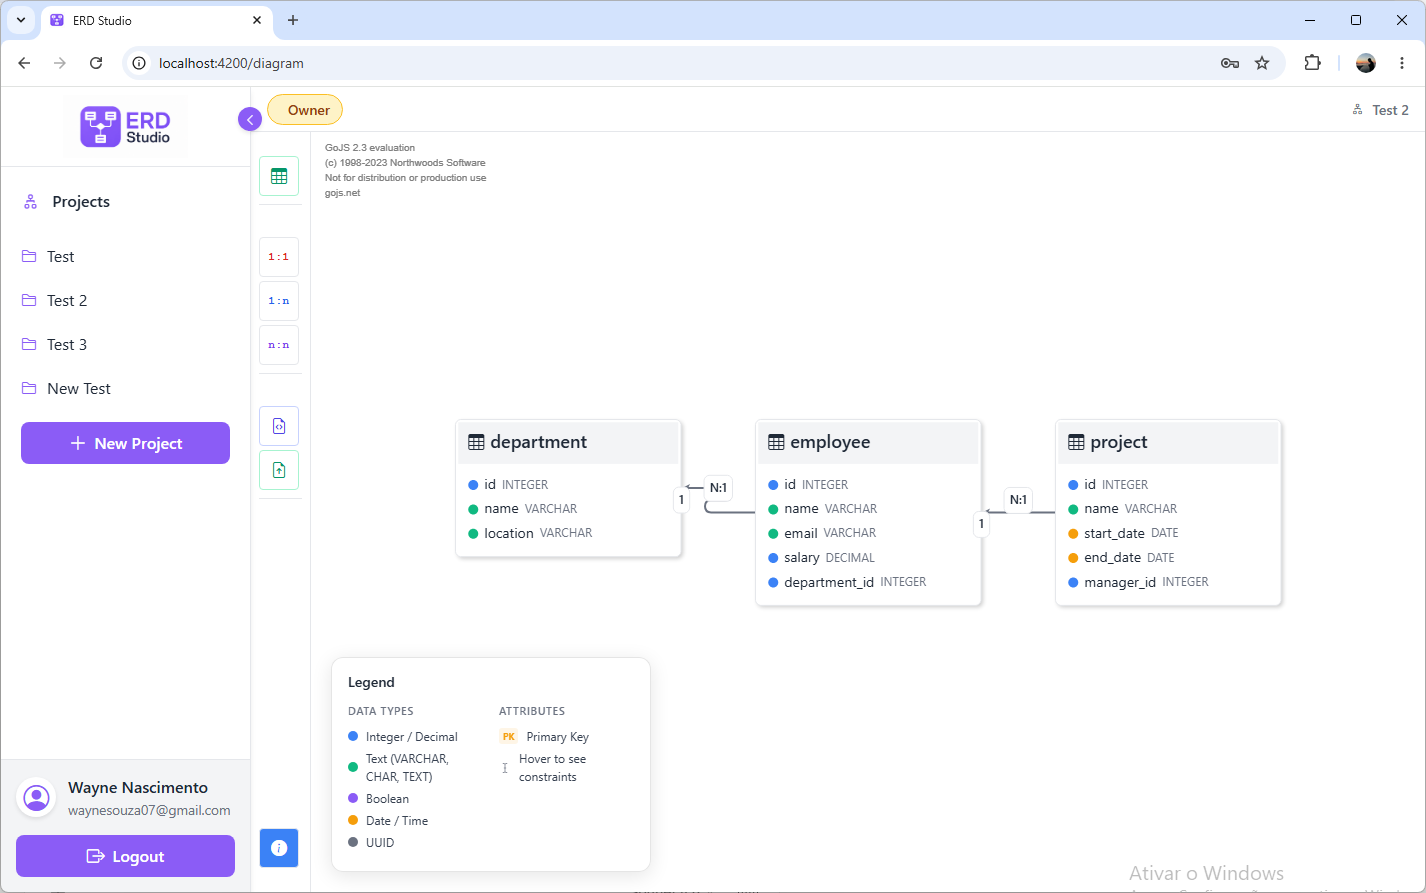
\includegraphics[width=15cm]{figuras/interface/tela-com-diagrama-simples-e-com-legenda.png}
    \caption{Editor de diagramas com legenda de tipos de dados}
    \begin{center}
        {\small Fonte: Elaborado pelo autor}
    \end{center}
    \label{fig:diagrama-com-entidades}
\end{figure}

Quando um usuário acessa um projeto com o papel de \textit{Viewer}, o editor é exibido em modo somente leitura. Conforme ilustra a Figura~\ref{fig:perfil-viewer}, a barra lateral de ferramentas é substituída por um indicador de visualização, impedindo qualquer operação de criação ou edição no diagrama. O papel atribuído ao usuário é exibido no topo da tela.

\begin{figure}[H]
    \centering
    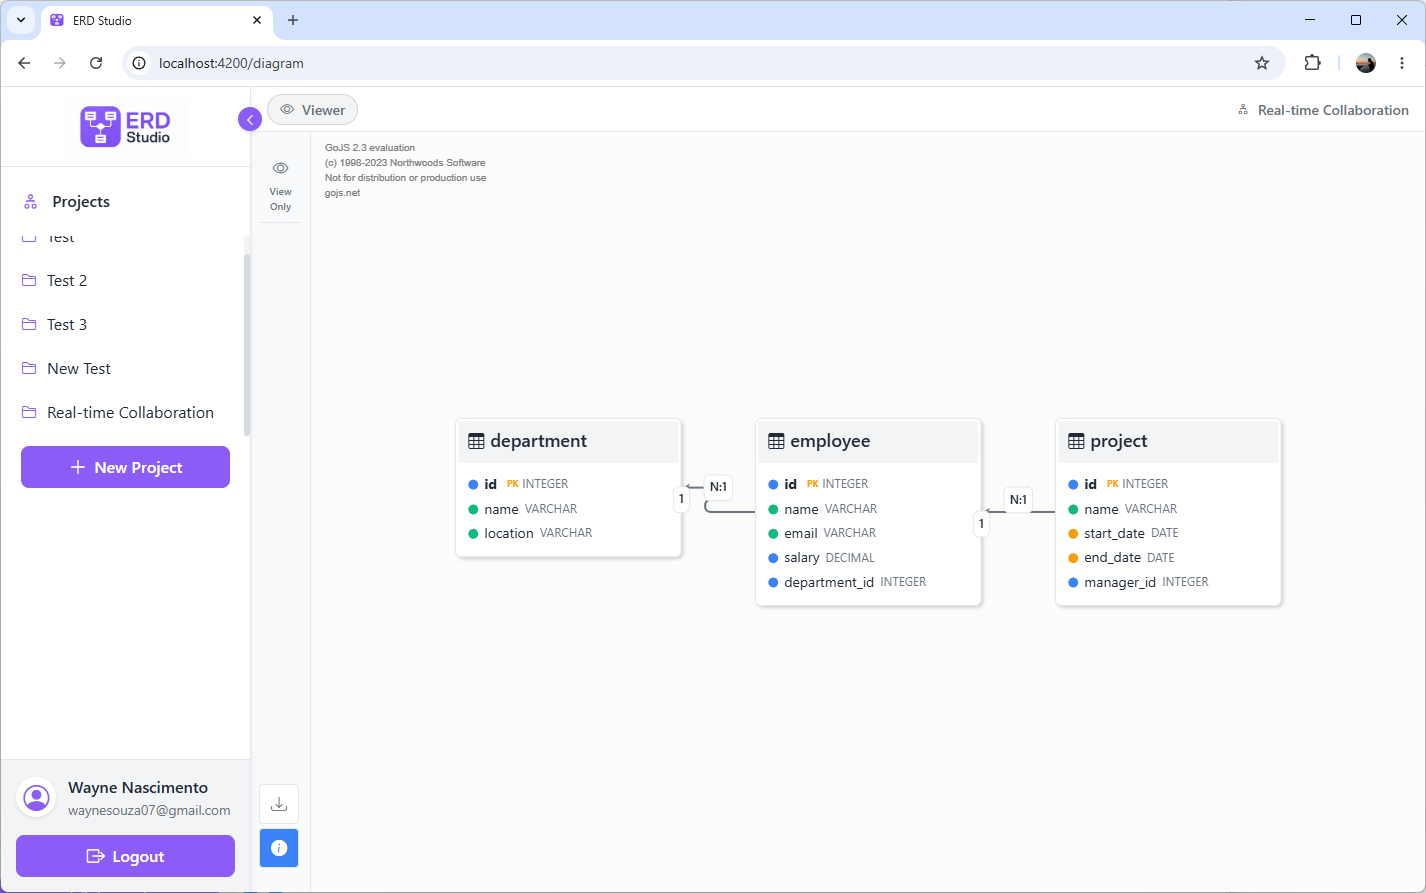
\includegraphics[width=15cm]{figuras/interface/tela-com-diagrama-simples-no-perfil-viewer.png}
    \caption{Editor de diagramas no perfil \textit{Viewer}}
    \begin{center}
        {\small Fonte: Elaborado pelo autor}
    \end{center}
    \label{fig:perfil-viewer}
\end{figure}

O mecanismo de bloqueio de entidades garante a consistência do diagrama durante sessões colaborativas simultâneas. Quando um colaborador inicia a edição de uma entidade, ela é bloqueada para os demais usuários conectados ao projeto. A Figura~\ref{fig:elemento-bloqueado} ilustra esse comportamento: a entidade \textit{employee} exibe uma borda tracejada indicando que está sendo editada por outro usuário, e uma notificação é exibida no topo da tela identificando o colaborador responsável pela edição.

\begin{figure}[H]
    \centering
    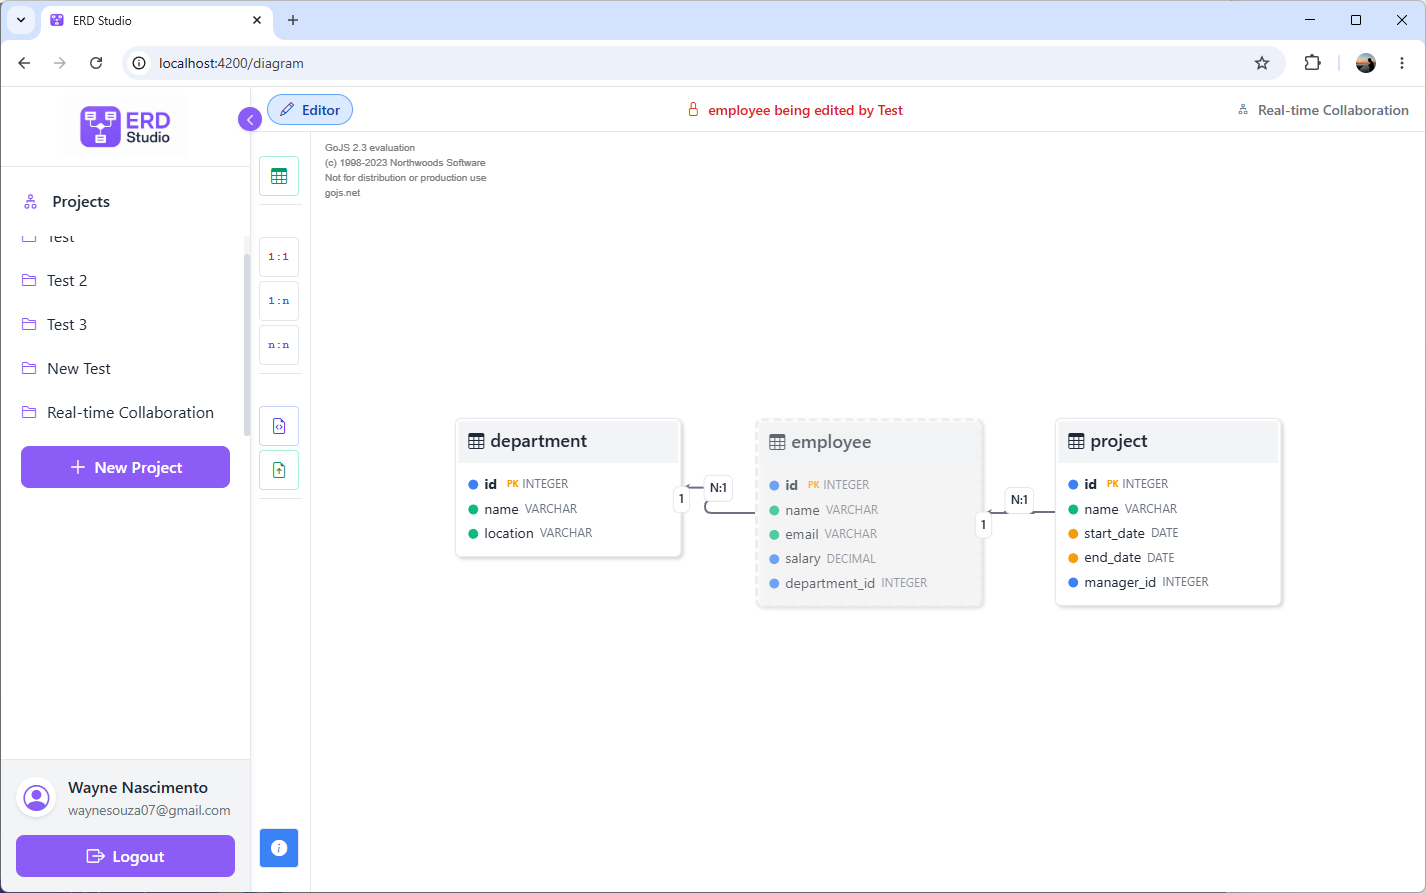
\includegraphics[width=15cm]{figuras/interface/tela-com-diagrama-simples-mostrando-elemento-bloqueado-por-outro-usuario.png}
    \caption{Entidade bloqueada por outro colaborador durante edição simultânea}
    \begin{center}
        {\small Fonte: Elaborado pelo autor}
    \end{center}
    \label{fig:elemento-bloqueado}
\end{figure}

\section{Disponibilidade do Código-Fonte e da Aplicação}

O código-fonte do protótipo está organizado em dois repositórios públicos no GitHub, separados por módulo:

\begin{itemize}
    \item \textbf{\textit{Back-end}:} \url{https://github.com/waynesouza/erd-core}
    \item \textbf{\textit{Front-end}:} \url{https://github.com/waynesouza/erd-client}
\end{itemize}

Após a implantação, a aplicação estará acessível temporariamente pelo navegador no seguinte endereço: \url{https://PLACEHOLDER_URL}. % TODO: substituir pela URL de deploy
